\chapter{Student Projects}\label{S:StudentProjects2007}
%\addcontentsline{toc}{chapter}{Student Project Appendix}
%Please visit: 
%\href{http://www.math.canterbury.ac.nz/~r.sainudiin/courses/STAT218/projects/Stat218StudentProjects2007.pdf}{\url{http://www.math.canterbury.ac.nz/~r.sainudiin/courses/STAT218/projects/Stat218StudentProjects2007.pdf}}\\
%and also visit: \href{http://www.math.canterbury.ac.nz/~r.sainudiin/courses/STAT218/projects/Stat218StudentProjects2008.pdf}{\url{http://www.math.canterbury.ac.nz/~r.sainudiin/courses/STAT218/projects/Stat218StudentProjects2008.pdf}} 
%
%to see the term projects completed by students of STAT 218 from 2007 and 2008.  Some of the simulation devices and non-perishable data from these projects are archived on the sixth floor of the Erskine Building.
Here are five examples of student projects. 
Students are strongly encouraged to work in teams of two or three. 
The projects are meant to encourage team-work. 
A student who wants to work on his or her own can do so. 
The following five student projects are model projects work the 5 bonus points. 
The project is completely optional and it is supposed to be an opportunity for learning certain important skills in mathematical and statistical communication. 


%%%%%%%%%%%%%%%%%%%%%%%%%%%%%%%%%%%%%%%%
%\newpage
\section{Testing the Approximation of $\pi$ by Buffon's Needle Test}
\begin{center}
Amanda Hughes \\and Sung-Lim Suh
\end{center}


%\begin{figure}
\begin{center}
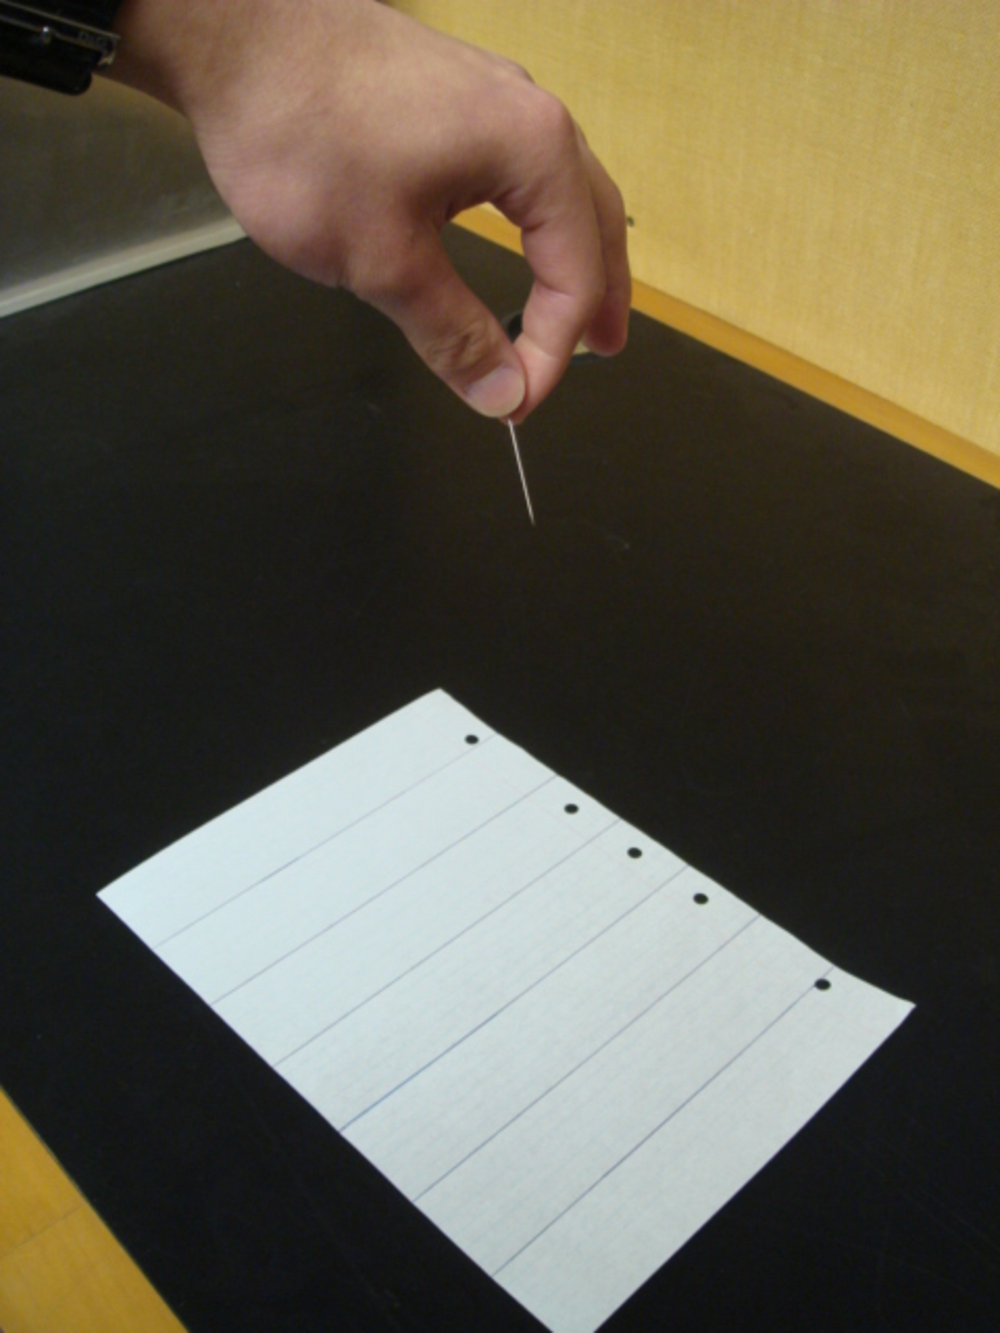
\includegraphics[width=4cm]{figures/BuffonNeedle_Drop}
\end{center}
%\end{figure}
%\end{abstract}


\subsection*{Abstract}

This project is designed to investigate Buffon's Needle experiment. We replicated the concept of Buffon's Needle and tested the null hypothesis that the outcomes from tossing a needle are directly related to $\pi$. The Delta Method and non-parametric methods have been employed in this project.

\subsection{Introduction \& Motivation}

The report will firstly cover the background and motivation of this project. Next we will explain the geometric background to why this experiment approximates $\pi$ and we will look at the statistical methodologies used. Following this we will discuss our results and conclusion. Finally we will discuss potential modifications.

\subsubsection*{Background - Comte de Buffon}

Comte de Buffon was born September 7 1707 in Montbard, France. He studied law in Dijon and medicine in Angers. After his studies, he had a chance to tour around France, Italy, and England to explore his knowledge in science. When he returned to France, Buffon published translations of one of Isaac Newton's works and his interest in science was now clear.

\subsubsection*{Background - Buffon's Needle}

Buffon's Needle Problem was first stated by Comte de Buffon in 1733, the solution was published later in 1777. The problem involves finding the probability that a needle of length $l$ will land on a line, given a floor with equally spaced parallel lines (or floorboards) a distance $d$ apart.

\subsubsection*{Motivation}

The motivation behind this project is to reconstruct Buffon's Needle Experiment. We wanted to see if an approximation of $\pi$ was found by this somewhat simple experiment over 200 years ago.

\subsection{Materials \& Methods}

\subsubsection*{Materials}

We first constructed a board which had several parallel lines. We did this by ruling lines on a piece of A4 paper. The width between the lines was either the same length as the needle or smaller than the length of the needle or larger than the length of the needle. The needle we used was a sewing needle of length 37mm. Instead of changing the needle to a smaller or larger needle for the three trials we ruled up three different sheets of A4 paper, one for each of the situations. The sheet that had the lines the same distance apart as the length of the needle had lines spaced 37mm apart. The sheet that had the lines closer together than the length of the needle had lines spaced 35mm apart. The sheet that had the lines further apart than the length of the needle had lines spaced 42mm apart. We recorded the data by entering it into Excel as the experiment was taking place. Sung-Lim tossed the needle and Amanda recorded the data.

\subsubsection*{Method}

We tossed a needle 200 times for each of the three different distances apart of the lines. Sung-Lim tossed the needle for all trials so that the tossing could be done as identically as possible. Sung-Lim held the needle at the same height and dropped it in exactly the same way for each trial. Sung-Lim called out each toss as either ``Yes" for the needle landing on a line or ``No" for the needle not landing on a line. Any decisions that had to be made over whether the needle crossed the line or not were made by Sung-Lim. If the needle rolled or bounced off the page we disregarded that trial. A break was taken every 100 trials so that all trials could be done as identically as possible.

\subsubsection*{Geometric Aspect}

We need to look at how this experiment approximates $\pi$. Let us begin by looking at the general case, where the needle is the same length as the distance between the floorboards.
\\
\\
Imagine a floor on which there are an infinite number of parallel lines (floorboards) spaced two units apart. You toss a needle that is also two units in length onto the floor. We want to find the probability that the needle crosses a line in the floorboards. $l$=the length of the needle and $d$=the distance between the lines.
\\
\begin{figure}[h]
\begin{center}
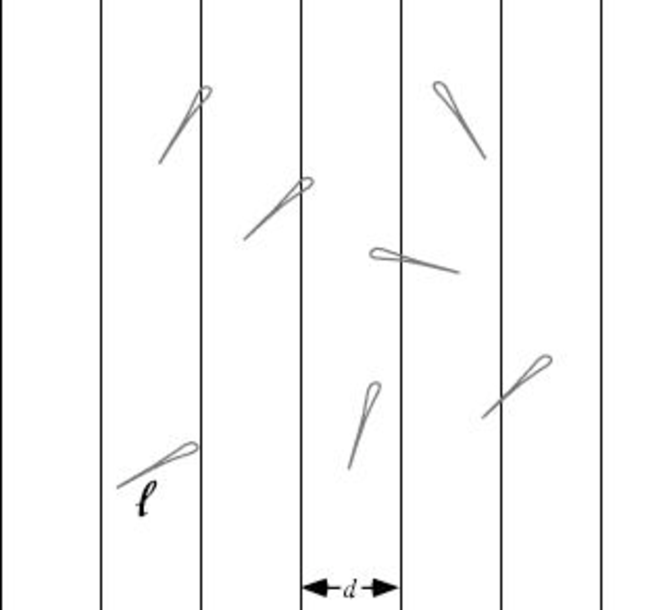
\includegraphics[width=6cm]{figures/BuffonNeedle_700}
\caption{Example of Needle Tosses}
\end{center}
\end{figure}


\begin{figure}[h]
\begin{center}
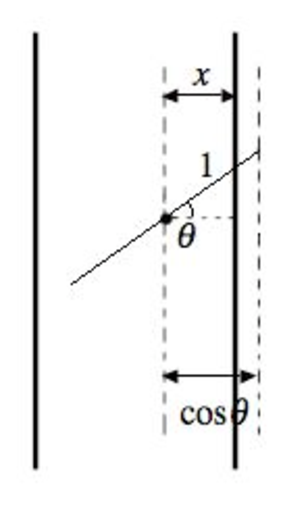
\includegraphics[width=4cm]{figures/BuffonNeedle_clip}
\caption{Explaining the outcomes of the needle toss}
\end{center}
\end{figure}

\noindent
Take one board to examine. Let $x$ be the shortest distance from the mid point of the needle to the nearest line. Let $\theta$ be the angle between $x$ and the needle. Imagine that there is a vertical line down from the end of the needle closest to the line. $\cos(\theta)$ gives the distance from the midpoint of the line to this imaginary line.\\
\\
As you can imagine, the needle can fall in an infinite amount of ways and positions relative to the parallel lines. Therefore, $\theta$ also has an infinite amount of possibilities. We will limit these possibilities in two ways. Firstly only consider the line that is closest to the midpoint of the needle. Secondly we will divide the board into two by drawing an imaginary line down the board halfway between two lines and only consider needle positions on the right side of our halfway line. We will consider the needles whose middle falls to the left of this imaginary line to be a rotation of the right side of the imaginary line. So we now only have two general situations to look at. One of these situations is shown in the above picture, where $\theta$ is less than $\pi/2$ radians. The other situation is where $\theta$ is larger than $\pi/2$ radians. In this case we will consider the angle $\theta$ to actually be the angle below of $x$ and we will think of this angle as negative. Therefore, the support of $x$ is 0 to 1 and the support of $\theta$ is $-\pi/2$ to $\pi/2$. This is shown in figure~\ref{BGC}.\\


\begin{figure}[h]
\begin{center}
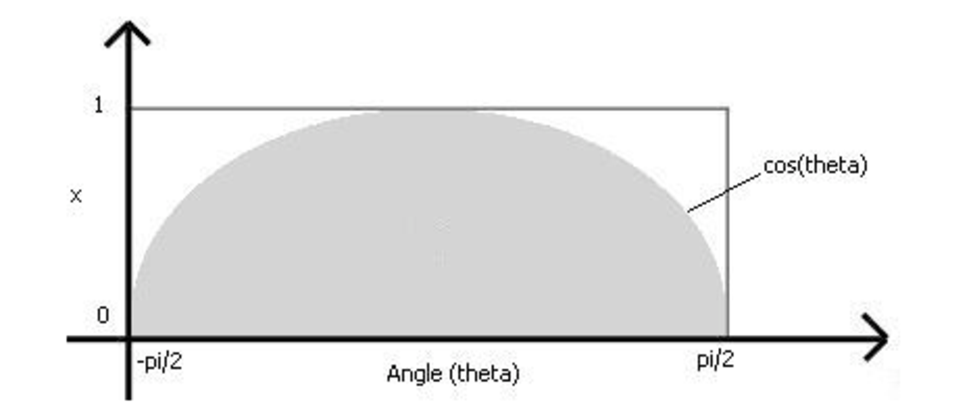
\includegraphics[width=12cm]{figures/BuffonNeedle_Cos}
\caption{Outcome Space of Buffon's Needle Experiment for General Case\label{BGC}}
\end{center}
\end{figure}

\noindent
The shaded area in figure~\ref{BGC}, represents when the needle crosses a line. This happens when
$x< \cos(\theta)$. The total outcome space is $\pi$ and the area under $\cos(\theta)$ from $-\pi/2$ to $\pi/2$ is 2 (integrating $\cos(\theta)$ from $-\pi/2$ to $\pi/2$). Therefore, the chance of a needle falling on a line is $2/\pi$.\\
\\
For the case where the needle is shorter in length than the distance between the floorboards we need to modify the above slightly. We need to account for the exact length difference between the needle and the floorboards. This is added to the above explanation by multiplying $2/\pi$ by $y$, which is the ratio of length of needle and distance between the lines, ie. $y=l/d$. Therefore the chance of a shorter needle landing on a line is $2y/\pi$.
\begin{displaymath}
\begin{array}{l}
\\\Pr(\text{needle crosses line})=\displaystyle\int^{2\pi}_0 (\frac{l|\cos\theta|}{d})\,\frac{d\theta}{2\pi}\\
\\\Pr (\text{needle crosses line}) =\displaystyle\frac{2l}{d\pi}\int^{\frac{\pi}{2}}_0 \cos\theta\,d\theta\\
\\\Pr (\text{needle crosses line}) =\displaystyle\frac{2l}{d\pi}\\
\\\Pr (\text{needle crosses line}) =\displaystyle\frac{2y}{\pi}\\
\end{array}
\end{displaymath}
\\
\noindent
For the case where the needle is longer in length than the distance between the floorboards we get a more complex outcome. We again need to account for the exact length difference between the needle and the floorboards. Therefore, the chance of a longer needle landing on a line is:
\begin{displaymath}
\begin{array}{l}
\\\Pr (\text{needle crosses line}) =\frac{2}{\pi}({y-\sqrt{y^2-1}+\sec^{-1}y})\\
\end{array}
\end{displaymath}

\subsubsection*{Statistical Methodology}

For this experiment we looked at the three different distances apart of the lines. For each of the three circumstances we used the same hypotheses.\\
H0(null hypothesis): $\phi^*=\frac{2}{\pi}$, the outcomes of tossing a needle are directly related to $\pi$\\
H1(alternative hypothesis): $\phi^*\neq\frac{2}{\pi}$, the outcomes of tossing a needle are not directly related to $\pi$\\
For the general case:
\begin{displaymath}
\begin{array}{l}
\\(\Theta,X)\overset{IID}{\sim} Uniform([\frac{\pi}{2},\frac{\pi}{2}] \times [0,1])\\
\end{array}
\end{displaymath}
as shown in figure 1.3. We know that for our simplest situation, where the length of the needle is the same as the distance between the lines:

\begin{displaymath}
\begin{array}{l}
\phi^*=\Pr((\Theta,X)\in \text{Shaded Region of figure~\ref{BGC}})=\frac{2}{\pi}\\
\\N_1,N_2,...,N_{200} \overset{IID}{\sim} Bernoulli(\phi^*)\\
\end{array}
\end{displaymath}
This is the probability of a needle landing on a line. The trials for each of the three different distances apart of the lines are 200 independent and identically distributed Bernoulli trials.
\\
\\
\noindent
Our maximum likelihood estimator of $\phi^*$ is:

\begin{displaymath}
\begin{array}{l}
\\\hat{\phi}_{200}=\frac{n_1+n_2+...+n_{200}}{200}\\
\end{array}
\end{displaymath}
This is the sample mean. But what we really want is a function of $\phi^*$, namely, $\Psi(\Phi):=2/\Phi$. We now need the Delta Method.  The Delta Method gives us the needed correction to transform an estimate and its  confidence interval.  By the Delta Method:
\[
\pi\approx\psi^*=g(\phi^*)=\frac{2}{\phi^*}
\]
and the maximum likelihood estimate of $\psi^*$ is:
\[
\hat{\psi}_{200}=g(\hat{\phi}_{200})=\frac{2}{\hat{\phi}_{200}}
\]
\noindent
Next we can calculate the standard error of our estimator of $\psi^*$, namely, $\hat{\Psi}_n=g(\hat{\Phi}_n)$, and subsequently confidence intervals:
\begin{displaymath}
\begin{array}{l}
\\se(\hat{\Psi}_n)=|g'( \phi)| se(\hat{\Phi}_n)\\
\\se(\hat{\Psi}_n)=|\frac{d}{d \phi}g( \phi)| se(\hat{\Phi}_n)\\
\\se(\hat{\Psi}_n)=|\frac{d}{d \phi}(2 \phi^{-1})| se(\hat{\Phi}_n)\\
\\se(\hat{\Psi}_n)=|-2 \phi^{-2}| se(\hat{\Phi}_n)\\
\\se(\hat{\Psi}_n)=(2 \phi^{-2}) se(\hat{\Phi}_n)\\
\end{array}
\end{displaymath}
where the estimated standard error is:
\begin{displaymath}
\begin{array}{l}
\\se(\hat{\psi}_{200})=(2 \phi_{200}^{-2}) se(\hat{\phi}_{200})=(2 \phi_{200}^{-2}) \frac{\hat{\phi}_{200} (1-\hat{\phi}_{200})}{200}\\
\end{array}
\end{displaymath}
Now we can calculate the 95\% confidence interval for $\psi^*\approx\pi$:
\begin{displaymath}
\begin{array}{l}
\\\hat{\psi}_{200}\pm1.96 se(\hat{\psi}_{200})\\
\end{array}
\end{displaymath}

Now for the needle shorter in length than the distance between the lines, where $\phi^*=\frac{2y}{\pi}$ and therefore by the Delta Method: $\pi\approx\frac{2y}{\phi^*}$, $\hat{\phi}_{200}$ is the sample mean of this set of data.
\begin{displaymath}
\begin{array}{l}
\\\psi^*=g(\phi^*)=\frac{2y}{\phi^*}\\
\\\hat{\Psi}_{200}=g(\hat{\phi}_{200})=\frac{2y}{\hat{\phi}_{200}}\\
\end{array}
\end{displaymath}
\noindent
From this we can calculate the standard error of the estimator of $\psi^*$, namely, $\hat{\Psi}_n$, and subsequently confidence intervals as follows:

\begin{displaymath}
\begin{array}{l}
\\se(\hat{\Psi}_n)=|g'( \phi)|*se(\hat{\Phi}_n)\\
\\se(\hat{\Psi}_n)=|\frac{d}{d \phi}g( \phi)|*se(\hat{\Phi}_n)\\
\\se(\hat{\Psi}_n)=|\frac{d}{d \phi}(2y \phi^{-1}|*se(\hat{\Phi}_n)\\
\\se(\hat{\Psi}_n)=|-2y \phi^{-2}|*se(\hat{\Phi}_n)\\
\\se(\hat{\Psi}_n)=(2y \phi^{-2})*se(\hat{\Phi}_n)\\
\end{array}
\end{displaymath}
\noindent
where the estimated standard error is
\begin{displaymath}
\begin{array}{l}
se(\hat{\psi}_n)=(2y \hat{\phi}_{200}^{-2})*se(\hat{\Phi}_n) \quad \text{and} \quad se(\hat{\Phi}_n)=\frac{\hat{\phi}_{200}*(1-\hat{\phi}_{200})}{200}\\
\end{array}
\end{displaymath}
Now we can calculate the 95\% confidence interval for $\psi^*\approx\pi$:
\begin{displaymath}
\begin{array}{l}
\\\hat{\psi}_{200}\pm1.96 se(\hat{\psi}_{200})\\
\end{array}
\end{displaymath}
\noindent
Now for the needle longer in length than the distance between the lines, where $\phi^*=\frac{2}{\pi}(y-\sqrt{y^2-1}+sec^{-1}y)$ and therefore by the Delta Method: $\pi\approx\frac{2}{\phi^*}(y-\sqrt{y^2-1}+sec^{-1}y)$, $\hat{\phi}_{200}$ is the sample mean of this set of data.

\begin{displaymath}
\begin{array}{l}
\\\psi^*=g(\phi^*)=\frac{2}{\phi^*}(y-\sqrt{y^2-1}+sec^{-1}y)\\
\\\hat{\psi}_{200}=g(\hat{\phi}_{200})=\frac{2}{\hat{\phi}_{200}}(y-\sqrt{y^2-1}+sec^{-1}y)\\
\end{array}
\end{displaymath}
\noindent
From this we can calculate the standard error of $\hat{\Psi}_{200}$, the estimator of $\psi^*$, and subsequently its confidence interval:

\begin{displaymath}
\begin{array}{l}
\\se(\hat{\Psi}_n)=|g'( \phi)| se(\hat{\Phi}_n)\\
\\se(\hat{\Psi}_n)=|\frac{d}{d \phi}g( \phi)| se(\hat{\Phi}_n)\\
\\se(\hat{\Psi}_n)=|\frac{d}{d \phi}\frac{2}{ \phi}(y-\sqrt{y^2-1}+sec^{-1}y)| se(\hat{\Phi}_n)\\
\\se(\hat{\Psi}_n)=|-2 \phi^{-2}| (y-\sqrt{y^2-1}+sec^{-1}y) se(\hat{\Phi}_n)\\
\\se(\hat{\Psi}_n)=(2 \phi^{-2}) (y-\sqrt{y^2-1}+sec^{-1}y) se(\hat{\Phi}_n)\\
\end{array}
\end{displaymath}

\noindent
where the estimated standard error is:
\begin{displaymath}
\begin{array}{l}
se(\hat{\Psi}_n)=(2 \hat{\phi}_{200}^{-2}) (y-\sqrt{y^2-1}+sec^{-1}y) se(\hat{\Phi}_n) \quad \text{and} \quad se(\hat{\Phi}_n)=\frac{\hat{\phi}_{200} (1-\hat{\phi}_{200})}{200}\\
\end{array}
\end{displaymath}
Now we can calculate the 95\% confidence interval for $\psi^*\approx\pi$:
\begin{displaymath}
\begin{array}{l}
\\\hat{\psi}_{200}\pm1.96 se(\hat{\psi}_{200})\\
\end{array}
\end{displaymath}

\subsection{Results}

For the needle same in length as the distance between the lines, we got an approximation for $\pi$ of  3.0769. The 95\% Confidence Interval (2.7640, 3.3898), contains $\pi$.\\
\\
For the needle shorter in length than the distance between the lines, we got an approximation for $\pi$ of 2.9122. The 95\% Confidence Interval (2.5861, 3.2384), contains $\pi$.\\
\\
For the needle longer in length than the distance between the lines, we got an approximation for $\pi$ of 2.8042. However, the 95\% Confidence Interval (2.5769, 3.0316), does not contain $\pi$.


\subsection{Conclusion}

For the first two cases the 95\% Confidence intervals both contain $\pi$ so we cannot reject the null hypothesis that the outcomes from tossing a needle are directly related to $\pi$. For the final case the 95\% Confidence interval does not contain $\pi$ so we reject the null hypothesis and conclude that for this case the outcomes from tossing a needle are not directly related to $\pi$. The first two outcomes agree with Buffon's Needle while the third one may in fact be false, because our samples were quite small in hindsight.


\subsubsection*{Potential Modification}

There are several ways we could improve this experiment. Firstly we could increase sample size and see if we can get better approximations of $\pi$. Secondly we could investigate the chance of a needle landing on a line on a square tiled floor, this is the Buffon-Laplace Needle. We could also extend the idea to not only cover needles and lines but also shapes and more complicated arrangements of tiles or lines.

\subsection*{Author Contributions}
\textbf{Amanda Hughes}

Original concept; research; recording of the data collection; MATLAB analysis; writing and construction of the report; LateX writing and compiling; some of the slides for presentation and some of the script for the presentation (mainly sections on the geometric aspect of the problem).

\noindent
\textbf{Sung-Lim Suh}

Research; collected data; majority of slides for presentation; majority of script for presentation, some of which was used in the report (Background on Comte de Buffon and Background of Buffon's Needle).
\\
\\
Many thanks to our lecturer Dr.~Raazesh Sainudiin who spent much of his time discussing the geometric aspect of this report with us. We really appreciated being able to stop by his office almost whenever and have a discussion.

\subsection*{References}

Texts:\\
Stigler,Stephen M.,\emph{Statistics on the Table: The History of Statistical Concepts and Methods}, Harvard University Press, USA, 2002\\
Electronic Texts:\\
Hyna, Irene; Oetiker, Tobias; Partl, Hubert; Schlegl, Elisabeth.,\emph{The Not so Short Introduction to LATEX 2e or LATEX 2e in 90 Minutes}, 2000\\
Websites:\\
\url{www.angelfire.com/wa/hurben/buff.html}\\
\url{www.mathworld.wolfram.com/BuffonsNeedleProblem.html}\\
\url{www.mste.uiuc.edu/reese/buffon/buffon.html}\\
\url{www.nndb.com/peopl/755/000091482/}\\
\url{www.ucmp.berkeley.edu/history/buffon2.html}\\
\url{www.youtube.com/watch?v=Vws1jvMbs64}\\

\subsection*{Appendix}

Data and MATLAB Code:

\VrbMf[label=Buffon.m]{scripts/Buffon.m}
%%%%%%%%%%%%%%%%%%%%%%%%%%%%%%%%%%%%%%%%
\newpage
\section{Estimating the Binomial probability p for a Galton's Quincunx}\label{S:AshmanLawrenceQuincunx}

\begin{center}
Bry Ashman and Ryan Lawrence
\end{center}

\subsection*{abstract}
Galton's Quincunx is a physical device designed to simulate the discrete binomial distribution. we aim to create a physical model of the quincunx that is characterised by the probability of a ball going left is equal to the probability of it going right. From the conceptual model of the quincunx, we derive the binomial probability mass function. In order to evaluate the parameter of interest \textit{p}, we will derive the maximum likelihood estimator and use this to estimate the actual parameter \textit{p} of our physical model using 100 samples that are assumed to be independent and identically distributed.
\begin{center}
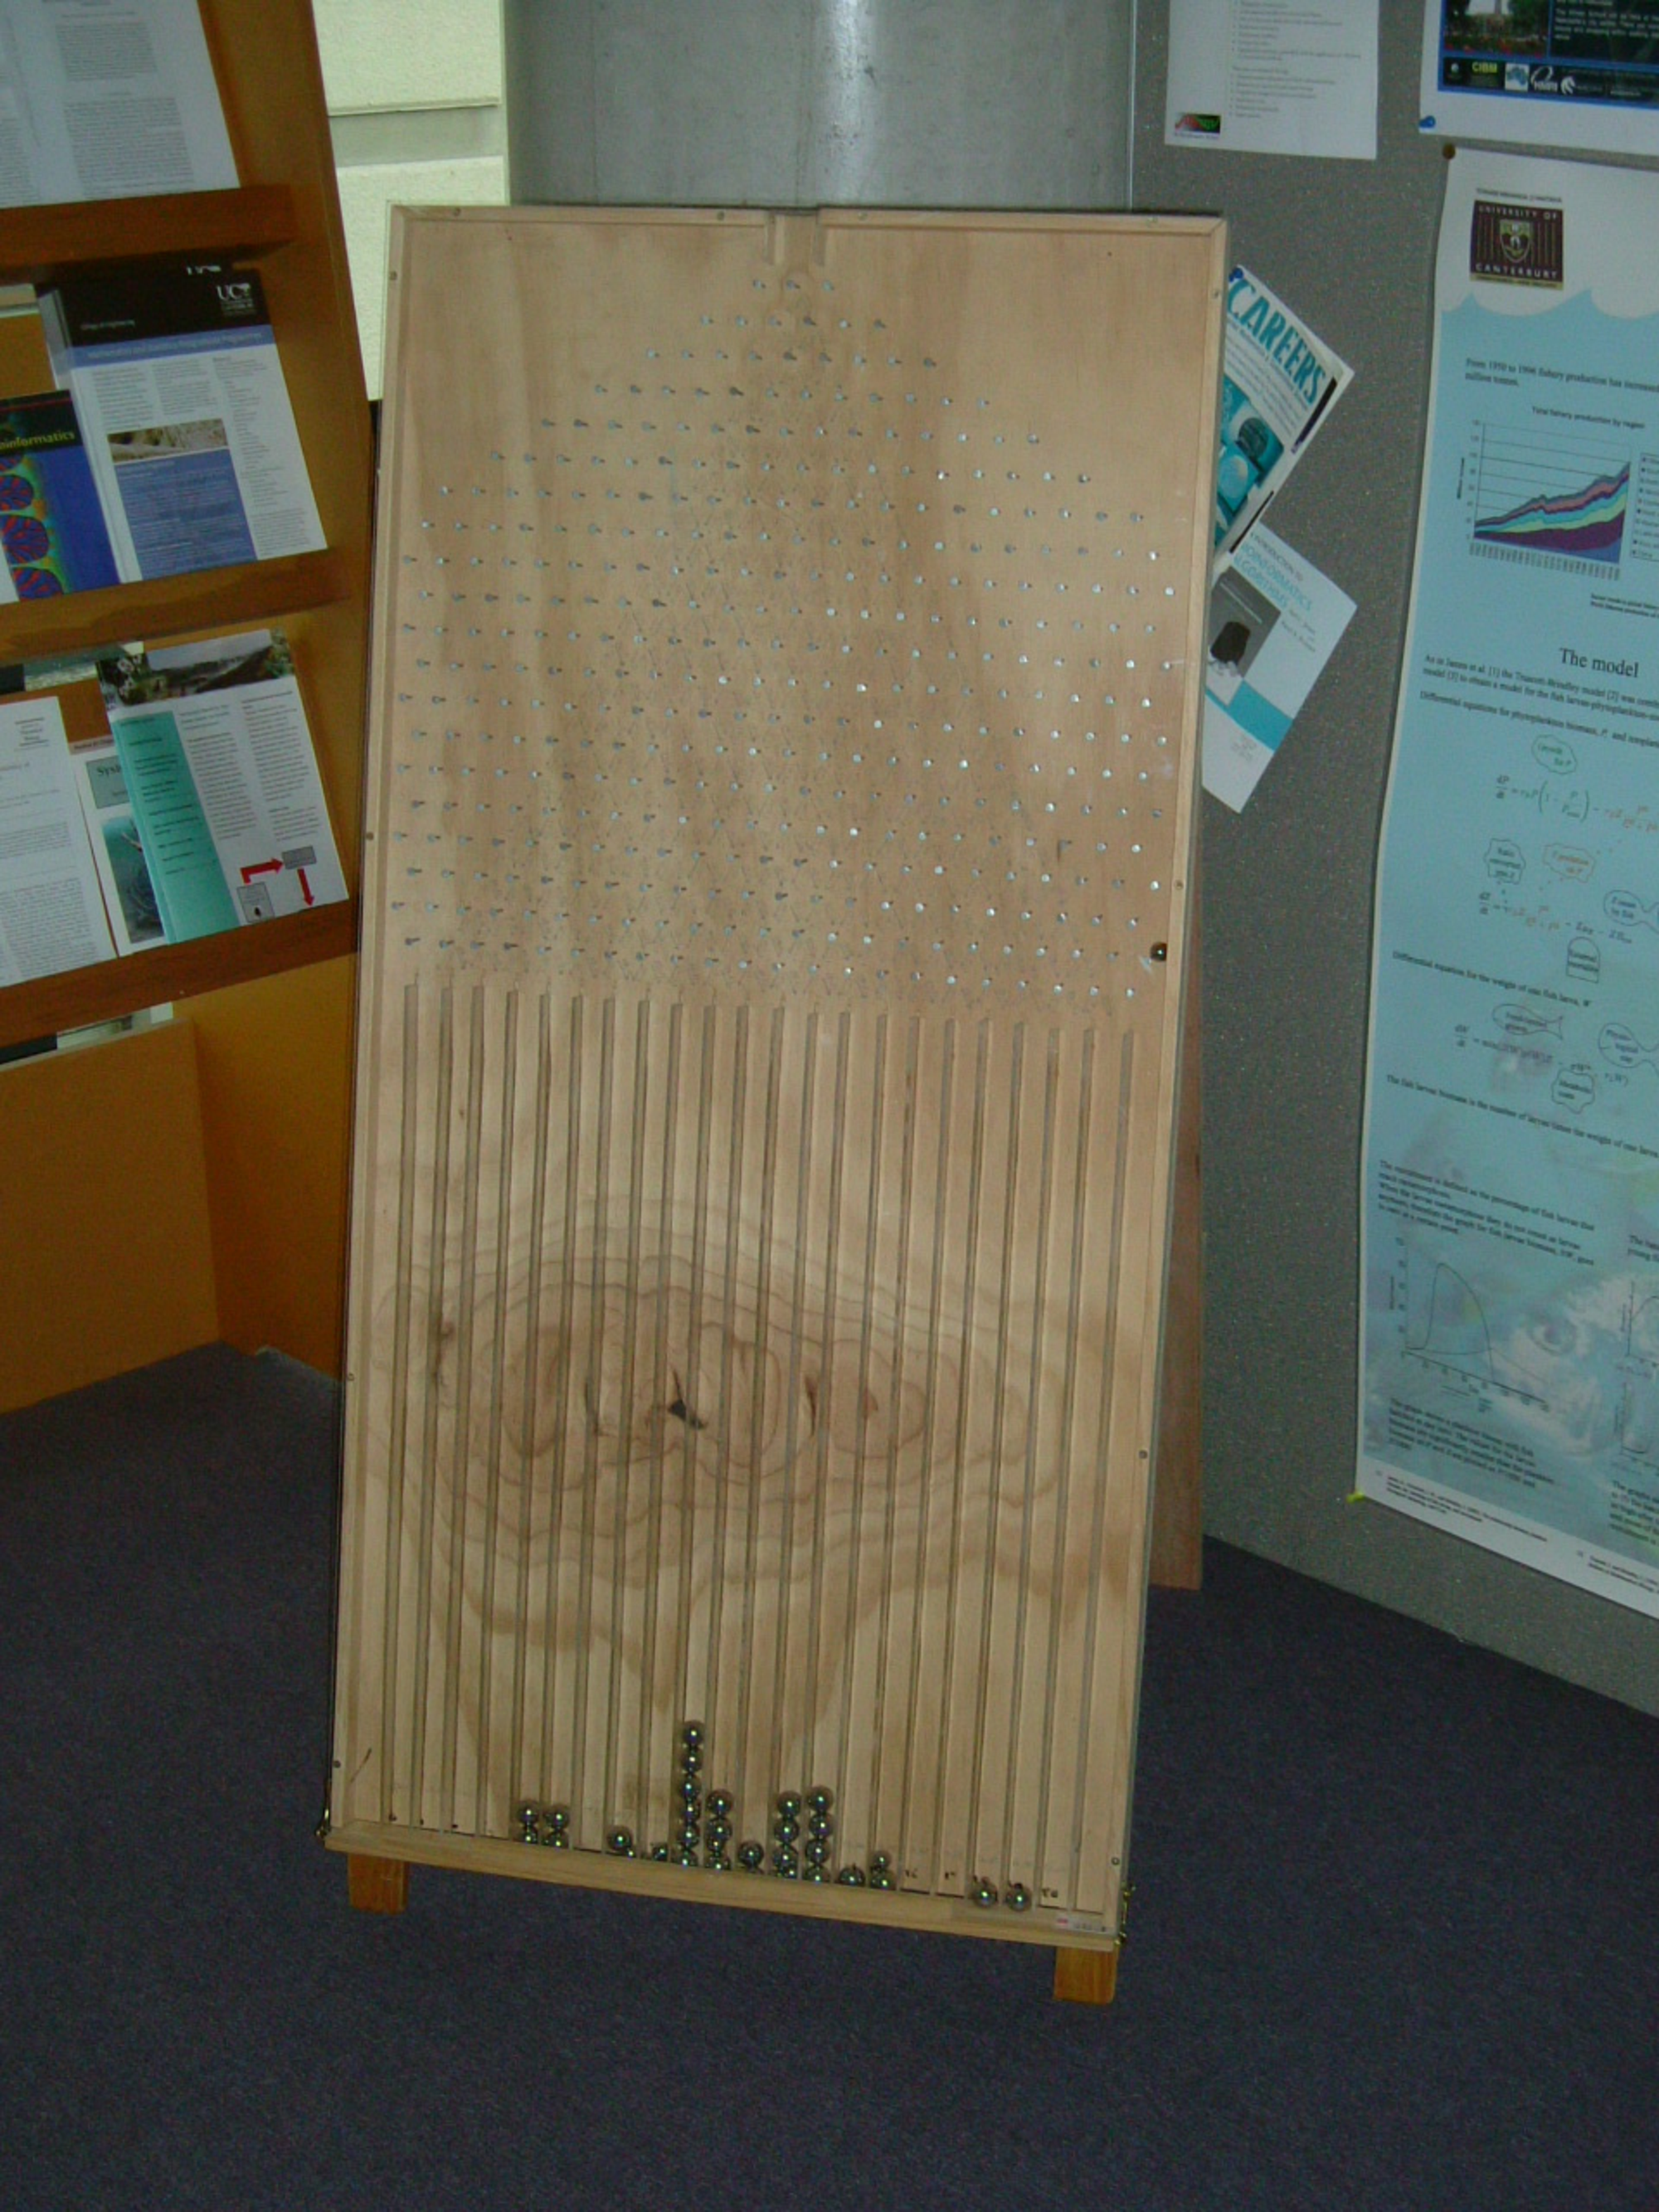
\includegraphics[width=8cm]{figures/AshmanLawrenceQuincunx.pdf}
\end{center}

%\newpage
\subsection{Motivation \& Introduction}
The binomial distribution is a fundamental discrete probability distribution, being the natural extension of the Bernoulli trial to the sum of Bernoulli trials. The distribution describes the number of successes in a sequence of $n$ binary trials, with a probability \textit{p}. Each of these trials is a Bernoulli trial parameterised by \textit{p}. A binomial distribution parameterised by $n=1$ and \textit{p} is simply a \textit{Bernoulli(p)} trial.

The quincunx was invented by Sir Francis Galton originally to demonstrate the normal distribution. The quincunx is simply an array of pegs spaced so that when a ball is dropped into a device, it bounces off the pegs with a prabability \textit{p} of going right and a probability of \textit{1-p} of going left. It bounces off $n$ pegs before being collected in a bin at the bottom of the device.

To this end, we aim to create a quincunx ideally parameterised by $p=0.5$ with $n=20$. To verify this, we will use maximum likelihood estimation to test the null hypothesis that $p=0.5$.

\subsection{Materials and Methods}
\subsubsection*{Construction of physical model}
The physical model that we created consisted of nails arranged in a pattern on a sheet of wood that we hoped would achieve as close to the ideal probability of p=0.5.

\subsubsection*{Materials}
\begin{itemize}
    \item Plywood Sheet (1200 x 600 x 20mm)
\item Perspex Sheets (1200 x 600 x 2mm and 550 x 800 x 2mm)
\item Timber Strips (1200 x 25mm and 600 x 25mm)
\item Nails (30 x 2mm)
\item Chrome Balls (20mm)
\end{itemize}


\subsubsection*{Construction Details}
\begin{enumerate}
    \item Mark 20 horizontal lines with 25mm spacings with the board in a portrait orientation.
\item Mark vertical lines at 25mm spacings from the centre of the board.
\item Place a nail at the top centre marking
\item Continue to place nails on the marked grid such that one marked grid point always separates the nails both vertically and horizontally.
\item Create the bins by attaching perspex strips directly below the nails of the last row.
\item Fit the edges to the main sheet. 
\item The perspex sheet can now be attached to the edges of the quincunx.
\end{enumerate}
 A desirable feature of the quincunx is a release mechanism at the top to release the balls used to simulate a random variable and a release at the bottom to retrieve the balls after the experiment.

\subsubsection*{Sample Collection}
To collect samples from the quincunx the balls are dropped into the device as identically as possible with sufficient time between each drop to ensure that the balls do not interfere with each other so as to keep the samples as identical as possible. The balls are collected in a series of bins numbered from 0 to 21, 0 representing the leftmost bin that the sample can be in and 21 being the rightmost bin. Since we assume that each sample is identical and independent, we record the cumulative number of balls in each bin after dropping 100 balls.
The data is shown in the blue bars in the next figure.

\begin{center}
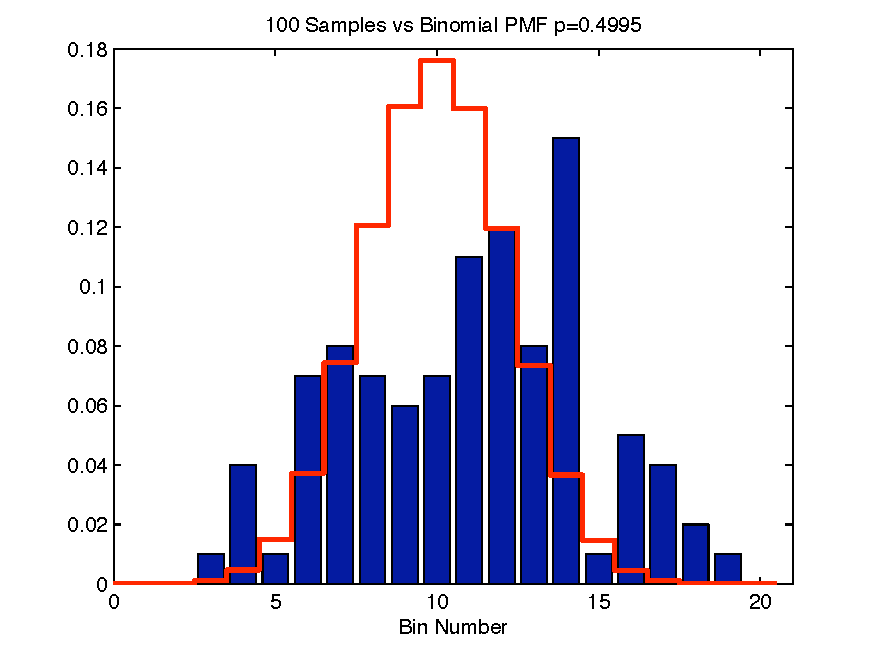
\includegraphics[width=9cm]{figures/AshmanLawrenceQuincunxData.pdf}
\end{center}

\subsection{Statistical Methodology}
\subsubsection*{Deriving the binomial distribution}
The binomial distribution can be thought of as a random walk in one dimension. The parameters map to this model as $p$ being the probability of taking a step right and $(1-p)$ the probability of taking a step left, and $n$ being the total number of steps taken. From this, it follows that, for a given number of $n$ steps, $x$ of which are to the right and $n-x$ to the left, to find the probability that a combination of those $n$ steps that will get you to the same point, you have to multiply the probability of the path by how many unique ways you can combine those steps. The number of ways of ordering the $x$ right steps in a set of $n$ steps is given by $(^n_x)$. Therefore, the probability of ending up at a particular endpoint is as follows: $$P(X=x)=\left(\begin{array}{c}n\\x\end{array}\right)p^x(1-p)^{n-x}$$
A note about the endpoint: I have used the convention that the leftmost bucket is 0. The end point numbers also tell you how many right steps you have in the quincunx.
\subsubsection*{Parametric Estimation}
In order to estimate the parameter $p$ for our physical model, we will use a maximum likelihood estimator (MLE) since it is often regarded as asymptotically optimal. However, for the binomial distribution, the MLE is equivalent to the Method of Moments.
\subsection*{Deriving the maximum likelihood estimator}
$$L(p)=\Pi^n_{i=1}\left(\begin{array}{c}N\\x_i\end{array}\right)p^{x_i}(1-p)^{N-x_i}$$
$$L(p)=\Pi^n_{i=1}\left(\begin{array}{c}N\\x_i\end{array}\right)p^{\Sigma x_i}(1-p)^{nN-\Sigma x_i}$$
$$lnL(p)=\Sigma^n_{i=1}ln\left(\begin{array}{c}N\\x_i\end{array}\right)\Sigma x_i ln(p)(nN-\Sigma x_i)ln(1-p)$$
$$\frac{d}{dp}lnL(p)=\frac{\Sigma x_i}{p}-\frac{nN-\Sigma x_i}{1-p}$$

We can now set $\frac{d}{dp}ln L(p)=0$ to find the maximum: $$0=\frac{\Sigma x_i}{p}-\frac{nN-\Sigma x_i}{1-p}$$
$$p=\frac{1}{nN}\Sigma^n_{i=1}x_i$$
Which is equivalent to:$$p=\frac{1}{N}E(X)$$
\subsection{Results \& Conclusion}
\subsubsection*{Maximum Likelihood Estimation}
The MLE of the parameter p of the quincunx is 0.4995, with a 95\% normal based confidence interval of [0.4639,0.5351] calculated as derived above.
\subsubsection*{Conclusion}
Maximum Likelihood Estimation from the 100 samples from the model of the quincunx has estimated the parameter for the binomial distribution to be in the range [0.4639,0.5351]. This would seem to verify that, in fact, even though the quincunx is a non-linear physical device that, overall, it is remarkably fair with p=0.5 within the 95\% normal based confidence interval.

The estimated cumulative distribution function also suggests that the distribution will converge binomially. Thus, we can conclude as $n\rightarrow \infty$, it will converge on the standard normal distribution as a consequence of the central limit theorem.
%%%%%%%%%%%%%%%%%%%%%%%%%%%%%%%%%%%%%%%%
\newpage
\section{Investigation of a Statistical Simulation from the 19th Century}
\begin{center}
Brett Versteegh and Zhu Sha
\end{center}
\subsubsection*{Abstract}
This project is designed to investigate Sir Francis Galton's statistical dice experiment. We constructed Galton's dice according to his prescriptions and tested the null hypothesis that the outcomes from these dice do indeed follow a discrete approximation to the normal distribution with median error one. The inverse distribution function sampler and Chi Squared test are the statistical methodologies employed in this project.

\begin{center}
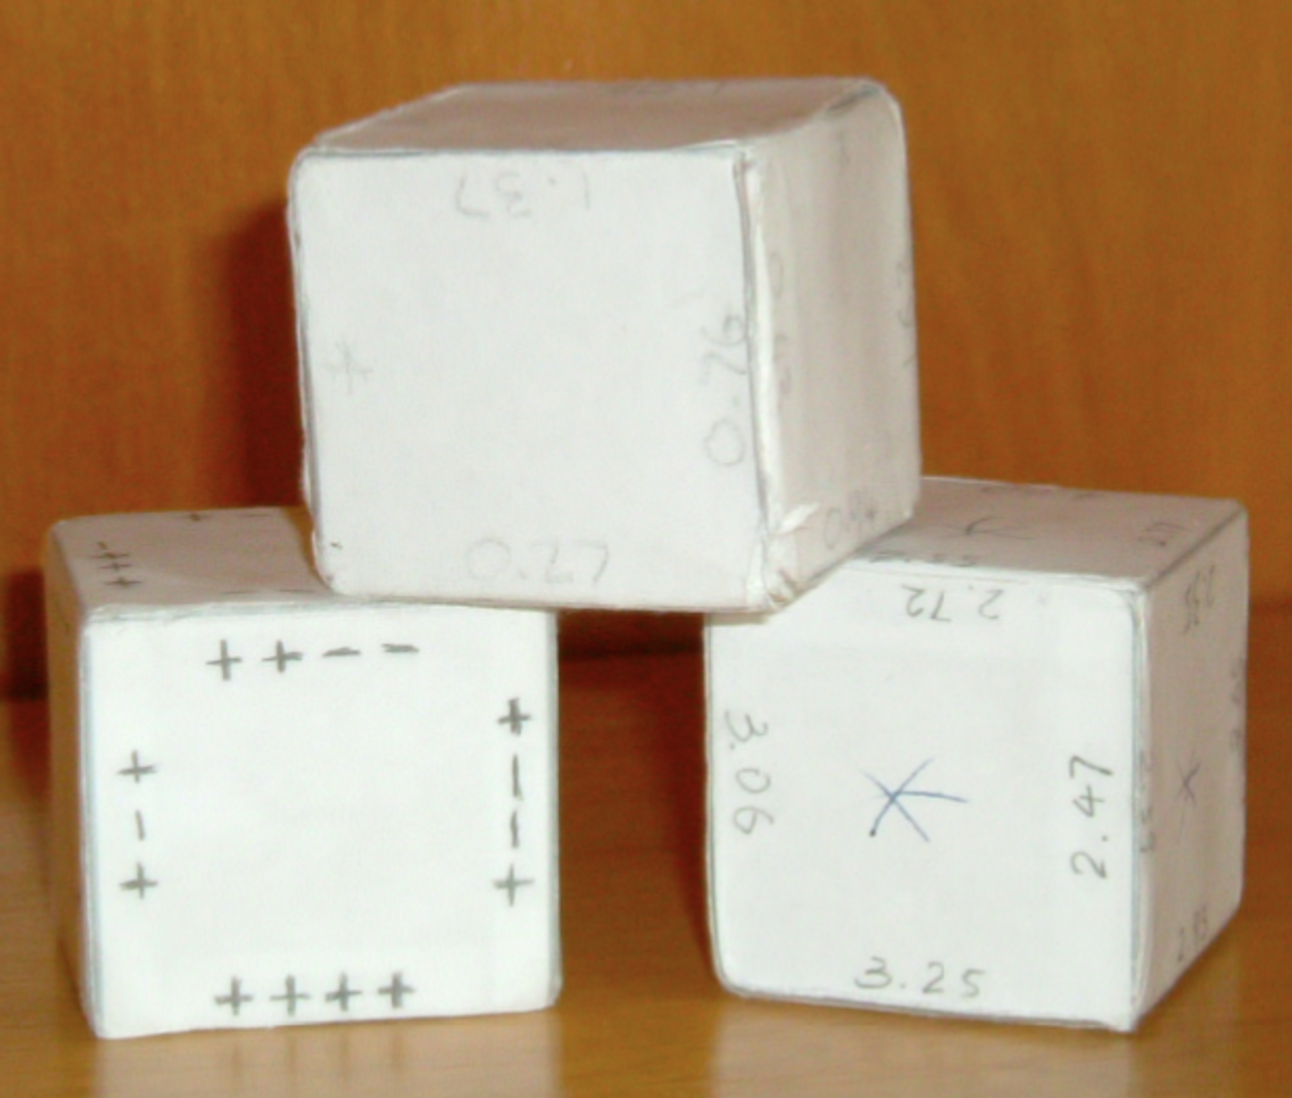
\includegraphics[width=4cm]{figures/GaltonDice.pdf}
\end{center}

\subsection{Introduction and Motivation}
The report will firstly cover the background and motivation of this project. Secondly, the methodologies used will be explained before outlining the results and subsequent conclusion found by undertaking this experiment. Finally, a potential modification to Galton's method will be examined as a means of sampling from a standard normal distribution.  

\subsubsection*{Francis Galton}
Born in 1822, Francis Galton was considered by many, at an early stage, to be a child prodigy. By the age of two, he could read; at five, he already knew some Greek, Latin and long division.

After his cousin, Charles Darwin, published \textit{The Origin of Species} in 1859, Galton became fascinated by it and thus devoted much of his life to exploring and researching aspects of human variation. Galton's studies of heredity lead him to introduce the statistical concepts of regression and correlation. In addition to his statistical research, Galton also pioneered new concepts and ideologies in the fields of meteorology, psychology and genetics.  

\subsubsection*{Statistical Dice}
This experiment came about from Galton's need, as a statistician, to draw a series of values at random to suit various statistical purposes. Dice were chosen as he viewed them to be superior to any other randomisation device. Cards and marked balls were too tedious to be continually shuffled or mixed following each draw, especially if the required sample size was large. 

The dice he created made use of every edge of each face which allowed for 24 equal possibilities as opposed to the six of a normal die.

For further details on Galton's experiment, please refer to his article \textquotedblleft Dice for Statistical Experiments\textquotedblright; \textit{Nature} (1890) No 1070, Vol 42 (This article is available free for download. Please refer to the references section for the website.)

\subsubsection*{Motivation}
The motivation behind this project is to reconstruct Galton's dice using the methods outlined in his 1890 \textit{Nature} article \textquotedblleft Dice for Statistical Experiments\textquotedblright and then harness the power of modern computers to determine how effective this technique was for simulating random numbers from the following distribution. 

Galton outlines that the samples were taken from a normal distribution with mean zero and median error one. We shall call this distribution Galton's Normal distribution or GN. However, for the experiment to work, we must use a discrete approximation of the normal distribution, which we will define as Galton's Discrete Normal or GDN. Both will be formally explained in the Methodology section. 

To determine the success of this experiment, we formulate the following question as a statistical hypothesis test:
\textquotedblleft Are our sampled values taken independently and identically from an appropriate discrete distribution which approximates Galton's normal distribution?\textquotedblright 


\subsection*{Materials and Methods}
\subsubsection*{Experiment Process}
In order to recreate Galton's Dice Experiment, we have chosen to replicate the design he explains in his \textit{Nature} article. 

\subsubsection*{Creating the Dice}
We chose to use rimu as it was readily available and inexpensive, unlike the mahogany that Galton had access to. As per his specifications, the wood was cut into six cubes of 1.25 inches (3.2 cm) wide, high and deep, before being covered in a paper template that was designed to fit tightly around the wood. The paper was adhered using general PVA glue. 

The only change to Galton's original specification was that we chose to write the values to two decimal places on the faces, as opposed to one decimal place. This was to ensure a higher level of precision when plotting the results. 

\subsubsection*{Collecting the Data}
The experiment was carried out by shaking all of the first three dice (dice 1) at once and rolling them across the flat surface of a table top. We interpreted Galton's terminology of the values that \textquotedblleft front the eye\textquotedblright to be the results that one can see by looking directly down on top of the dice. The three dice were then lined up into a row and the values called out and entered onto a Notepad document. We used the following formula to calculate the optimal number of trials needed for our investigation:$f(x)_{min}*sample\textrm{ }size\approx 5 $, where $f(x)_{min}$ is the smallest probability for the discrete distribution. 

The same rolling process was then performed for dice 2 (two dice at once) and 3 (only one die) with the single exception that we did not need to roll these dice as many times as dice 1. 


 
\subsection{Statistical Methodology}
Firstly, we will define Galton's Normal distribution. As derived from an article published in \textit{Statstical Science}\footnote[1]{Stochastic Simulation in the Nineteenth Century. {\it Statistical Science} (1991) Vol 6, No 1, pg 94.}, Galton's Normal Distribution has a mean of zero but the variance is not one. Instead, Galton's sample is taken from a half-normal distribution with a \textquotedblleft probable error\textquotedblright (median error) of one. This implies that the probability between zero and one is a quarter, allowing us to solve the following equation to determine the variance: 
\begin{displaymath}
\begin{array}{l}
\phi(x)=\frac{1}{\sigma\sqrt{2\pi}}exp(-\frac{x^2}{2\sigma^2})\\
\frac{1}{4}=\int_0^1\phi(x)dx\\
\frac{1}{4}=\int_0^1\frac{1}{\sigma\sqrt{2\pi}}exp(-\frac{x^2}{2\sigma^2})dx\\
\sigma=1.4826
\end{array}
\end{displaymath}

$ \therefore $ GN $\sim$ N (0, 1.48262)

Secondly, we must determine how Galton calculated the values\footnote[2]{See Appendix B.} to use on his dice. It was our assumption that he used the midpoints of a set of intervals that partition [0, 1] and we undertook the following processes to confirm this. 

We divided the interval [0.5 1] equally into 24, with the last 3 intervals further divided into 24 subintervals. In total, this gave us 21 + 24 intervals to allocate along the y-axis. The midpoint of each interval was taken in order to compute its corresponding $x$ value under the inverse CDF map.

\begin{figure}[thp]
\begin{center}
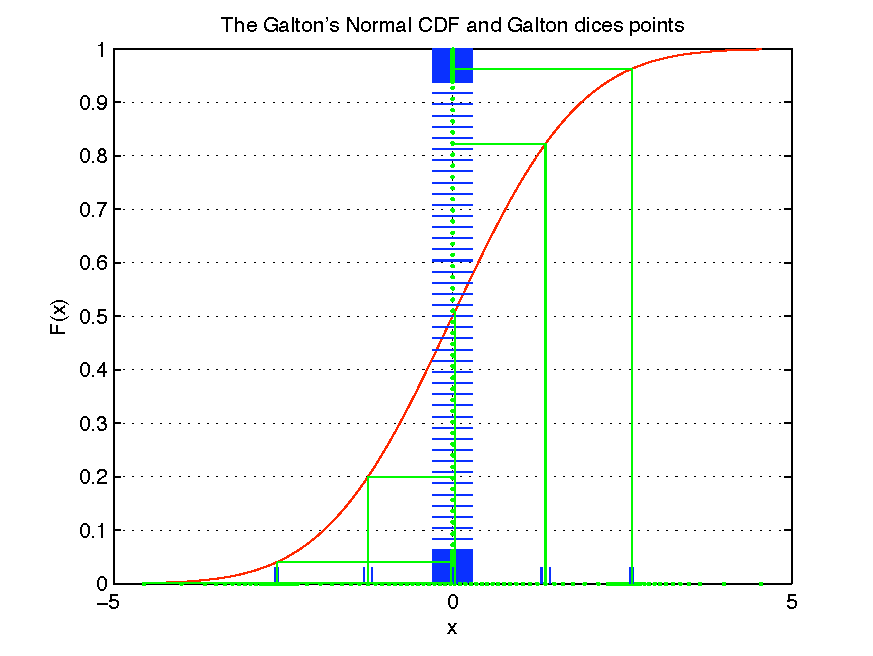
\includegraphics[width=10cm]{figures/GaltonDice_normal_cdf_and_galton_dices_points.pdf}
\caption{Plot showing the midpoints mapping back to specific values on the x axis.}
\end{center}
\end{figure}

The easiest way to do this would have been to evaluate the inverse CDF function at the midpoints. However, a closed form expression for the inverse CDF does not exist for a Normal distribution. Thus, we applied numerical methods to solve for $x$ (Newton's method).  

We believe the midpoint assumption was correct, as the mapped values are very close to Galton's actual figures and the differences can be attributed to an imprecise value for the standard deviation. 

Thirdly, we can now determine Galton's discrete approximation to the Normal. This is necessary as the values drawn from throwing Galton's dice come from a discrete distribution, not the continuous Galton Normal. In doing this, we are also able to define our null hypothesis formally: \textbf{$H_0: x_1, x_2,\ldots, x_n IID \sim GDN$}
Galton's Discrete Normal (GDN) is an approximation to Galton Normal (GN).

\begin{figure}[thp]
\begin{center}
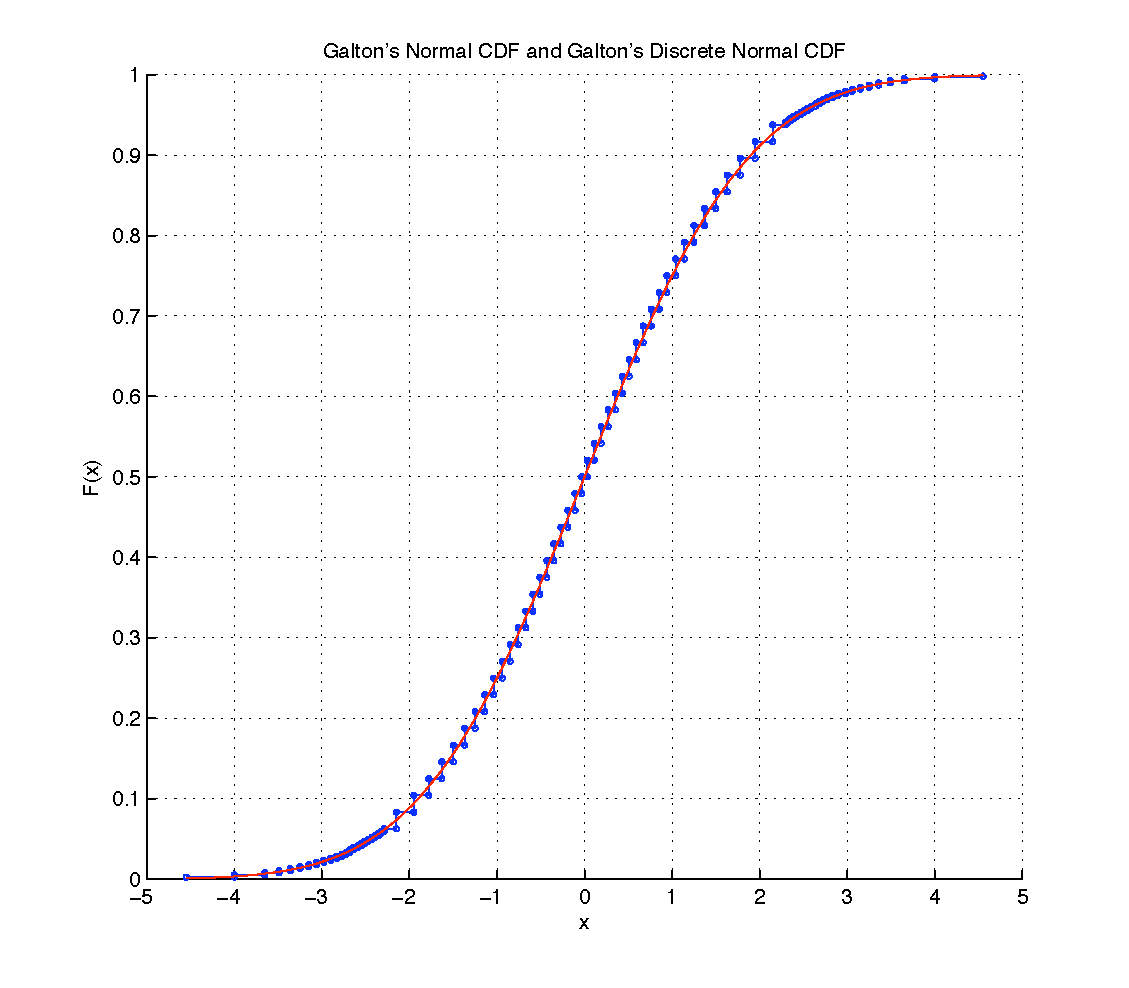
\includegraphics[width=10cm]{figures/GaltonDice_Normal_CDF_and_Galtons_Discrete_Normal_CDF.pdf}
\caption{Plot showing both the GN and GDN CDFs. They are very similar.}
\end{center}
\end{figure}
 

Fourthly, as the distribution is now discrete, we can apply the Chi Squared Test to evaluate our null hypothesis. The test used had the following parameters:
Degrees of Freedom: $90 -1 = 89$ 
 $\alpha = 0.05$;
Critical Value = 112.

\subsection{Results}
Once the experiment was complete and the results collated, they were run through a methodological tester to ensure all values were correct. Testing the data involved running all our sampled values through a {\tt Matlab} function which checked each number against Galton's 45 possible values. Any values that did not match were outputted as ones and the erroneous data were removed before a graph was plotted to measure how well our experiment sampled from GDN. 

\begin{figure}[thp]
\begin{center}
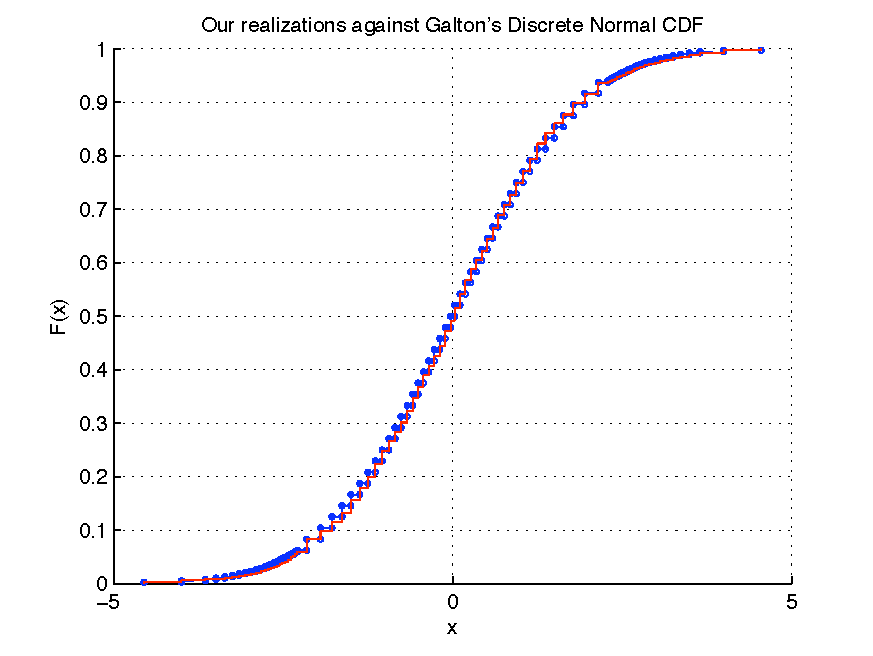
\includegraphics[width=10cm]{figures/GaltonDice_our_realizations_against_Galtons_discrete_normal.pdf}
\caption{Plot showing the empirical DF of our results against GDN. Our values take on a stair case appearance and are very close to GDN. The main deviations occur mostly in the tails.}
\end{center}
\end{figure}
  

\subsubsection*{Chi Squared Test}
A Chi Squared test was then performed on the data and the results\footnote{For the full table, please see Appendix A.} are summarised below. 
	
\begin{tabular}{|c|c|c|c|c|}\hline
&Data Values	&Observed Count&	Expected Count&	$(O-E)^2/E$\\ \hline
	&-4.55	&5&	5.046875&	0.000435372\\
	&-4&	7	&5.046875&	0.755853328\\
	&-3.65	&5&	5.046875&	0.000435372\\
	&3.49&	6	&5.046875	&0.180001935\\
	&\ldots &	\ldots&\ldots&\ldots\\
	&3.65&	8	&5.046875	&1.727989551\\
	&4	&11	&5.046875&7.022107198\\
	&4.55&	5	&5.046875	&0.000435372\\
Total	&& 	1938	&1938	 &\\\hline
Chi Test Result	 	 &&&&	 	83.54798762\\\hline
\end{tabular}



$$T=\Sigma_{i=1}^{90} \frac{(Obseverd-Expected)^2}{Expected} = 83.548$$

\begin{figure}[thp]
\begin{center}
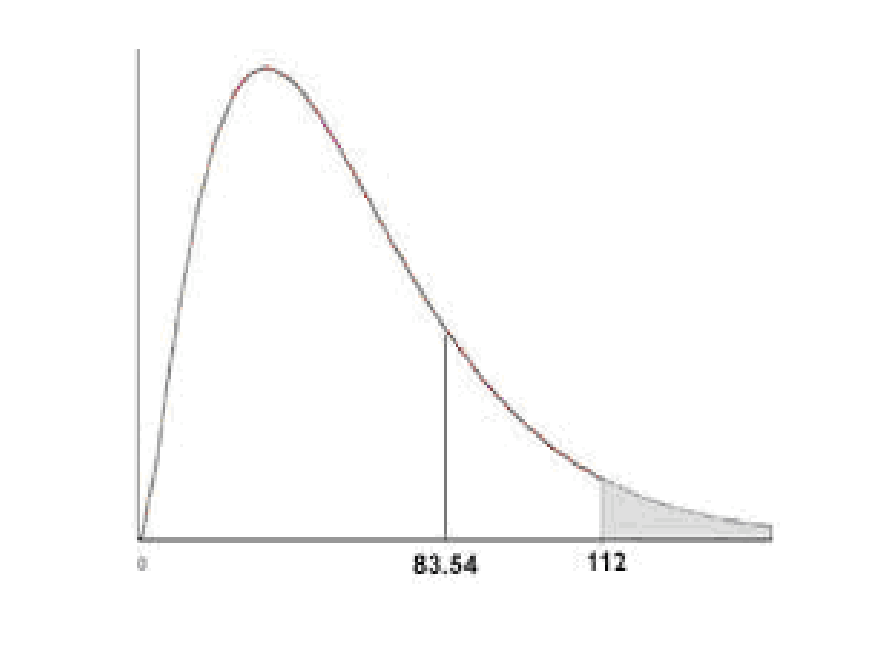
\includegraphics[width=6cm]{figures/GaltonDice_chisquare.pdf}
\end{center}
\end{figure}
 

\subsection{Conclusion}
We cannot reject H0 at   = 0.05 because the observed test statistic is outside the rejection region. In relation to our statistical question, this means that there is insufficient evidence to suggest that our sample is not from GDN. 

 
\subsubsection*{Potential Modification}
Since the standard normal distribution is more common in all areas, we wanted to convert Galton's Dice into a new set which can be used for simulating the standard normal distribution. 

In his experiment, Galton took the mid-point of each probability interval, and then found the corresponding $x$- values. Instead of applying a tedious calculation to find the $x$-values, we took a $z$-value table, and found the corresponding $z$-values to the upper bound of those intervals. This enables the creation of two new dice\footnote{Tables showing the new values for dice 1 \& 2. The third dice can remain the same as Galton's.}:
\newline

Dice (1)
\begin{tabular}{|cccccc|}\hline
0.05	&0.10	&0.15&	0.21&	0.27&	0.32\\
0.37&	0.43&	0.49&	0.55&	0.61&	0.67\\
0.74	&0.81&	0.89&	0.97&	1.05&	1.15\\
1.26	&1.38	&1.53& 	*&	*&	*\\\hline
\end{tabular}


Dice (2)
\begin{tabular}{|cccccc|}\hline
1.56&	1.58&	1.60&	1.62&	1.65&	1.68\\
1.70	&1.73&	1.76&	1.79&	1.83&	1.86\\
1.90&	1.94	&1.99	&2.04&	2.09	&2.15\\
2.23	&2.31	&2.42&	2.56&	2.80	&4.00\\\hline
\end{tabular}




Through {\tt Matlab}, we were able to map the data gathered during our original experiment into the values shown in previous table, corresponding to the standard Normal, and develop the following plot: 

\begin{figure}[thp]
\begin{center}
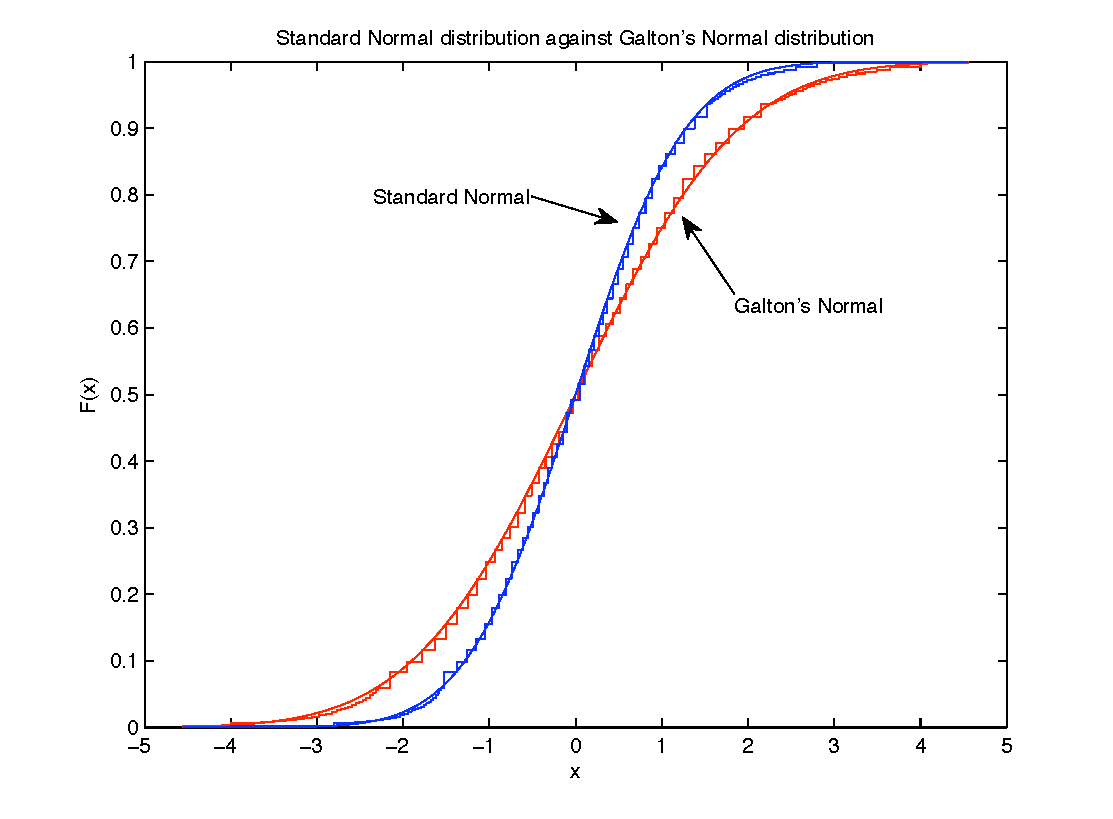
\includegraphics[width=10cm]{figures/GaltonDice_standardnormal_against_galtons_normal.pdf}
\caption{Plot showing the Standard Normal Distribution against Galton's Normal Distribution.}
\end{center}
\end{figure}


%\newpage
\subsection*{Author Contributions}
\textbf{Brett} - Constructed dice, gathered majority of the data results, constructed report, conducted spell/grammar check.

\noindent
\textbf{Joe} - Wrote up {\tt Matlab} code to analyse and plot data, entered in data results, constructed presentation and discovered a modification to Galton's experiment.  


\subsection*{References}
Dice for Statistical Experiments. $Nature$ (1890) Vol 42, No 1070

\noindent
Stochastic Simulation in the Nineteenth Century. $Statistical Science$ (1991) Vol 6, No 1

\noindent
\url{http://www.galton.org}

\noindent
\url{http://www.anu.edu.au/nceph/surfstat/surfstat-home/tables/normal.php}

%\newpage
\subsection*{Appendix A}
\renewcommand{\baselinestretch}{1}
\begin{center}
{\scriptsize
\begin{tabular}{|c|c|c|c|}\hline
Data	& Count&	Expected Count&	$(O-E)^2/E$\\ \hline
-4.55	&	5	&	5.046875	&	0.000435372	\\
-4	&	7	&	5.046875	&	0.755853328	\\
-3.65	&	5	&	5.046875	&	0.000435372	\\
-3.49	&	1	&	5.046875	&	3.245017415	\\
-3.36	&	3	&	5.046875	&	0.830156734	\\
-3.25	&	3	&	5.046875	&	0.830156734	\\
-3.15	&	3	&	5.046875	&	0.830156734	\\
-3.06	&	4	&	5.046875	&	0.217153638	\\
-2.98	&	4	&	5.046875	&	0.217153638	\\
-2.9	&	3	&	5.046875	&	0.830156734	\\
-2.83	&	8	&	5.046875	&	1.727989551	\\
-2.77	&	5	&	5.046875	&	0.000435372	\\
-2.72	&	3	&	5.046875	&	0.830156734	\\
-2.68	&	3	&	5.046875	&	0.830156734	\\
-2.64	&	3	&	5.046875	&	0.830156734	\\
-2.59	&	6	&	5.046875	&	0.180001935	\\
-2.55	&	4	&	5.046875	&	0.217153638	\\
-2.51	&	5	&	5.046875	&	0.000435372	\\
-2.47	&	4	&	5.046875	&	0.217153638	\\
-2.43	&	6	&	5.046875	&	0.180001935	\\
-2.39	&	10	&	5.046875	&	4.861116486	\\
-2.35	&	6	&	5.046875	&	0.180001935	\\
-2.32	&	8	&	5.046875	&	1.727989551	\\
-2.29	&	6	&	5.046875	&	0.180001935	\\
-2.15	&	47	&	40.375	&	1.087074303	\\
-1.95	&	28	&	40.375	&	3.792956656	\\
-1.78	&	34	&	40.375	&	1.006578947	\\ 
-1.63	&	33	&	40.375	&	1.347136223	\\
-1.5	&	45	&	40.375	&	0.529798762	\\
-1.37	&	46	&	40.375	&	0.783668731	\\
-1.25	&	37	&	40.375	&	0.282120743	\\
-1.14	&	48	&	40.375	&	1.44001548	\\
-1.04	&	48	&	40.375	&	1.44001548	\\
-0.94	&	35	&	40.375	&	0.715557276	\\
-0.85	&	34	&	40.375	&	1.006578947	\\
-0.76	&	34	&	40.375	&	1.006578947	\\
-0.67	&	41	&	40.375	&	0.009674923	\\
-0.59	&	49	&	40.375	&	1.84249226	\\
-0.51	&	37	&	40.375	&	0.282120743	\\
-0.43	&	44	&	40.375	&	0.325464396	\\
-0.35	&	33	&	40.375	&	1.347136223	\\
-0.27	&	36	&	40.375	&	0.474071207	\\
-0.19	&	36	&	40.375	&	0.474071207	\\
-0.11	&	55	&	40.375	&	5.297600619	\\
-0.03	&	38	&	40.375	&	0.139705882	\\
0.03	&	45	&	40.375	&	0.529798762	\\
\hline
\end{tabular}
}
%\newpage
{\scriptsize
\begin{tabular}{|c|c|c|c|}\hline
Data	& Count&	Expected Count&	$(O-E)^2/E$\\ \hline
0.11	&	53	&	40.375	&	3.947755418	\\
0.19	&	48	&	40.375	&	1.44001548	\\
0.27	&	40	&	40.375	&	0.003482972	\\
0.35	&	35	&	40.375	&	0.715557276	\\
0.43	&	32	&	40.375	&	1.737229102	\\
0.51	&	42	&	40.375	&	0.065402477	\\
0.59	&	41	&	40.375	&	0.009674923	\\
0.67	&	46	&	40.375	&	0.783668731	\\
0.76	&	35	&	40.375	&	0.715557276	\\
0.85	&	38	&	40.375	&	0.139705882	\\
0.94	&	45	&	40.375	&	0.529798762	\\
1.04	&	44	&	40.375	&	0.325464396	\\ 
1.14	&	43	&	40.375	&	0.170665635	\\
1.25	&	55	&	40.375	&	5.297600619	\\
1.37	&	38	&	40.375	&	0.139705882	\\
1.5	&	35	&	40.375	&	0.715557276	\\
1.63	&	32	&	40.375	&	1.737229102	\\
1.78	&	42	&	40.375	&	0.065402477	\\
1.95	&	33	&	40.375	&	1.347136223	\\
2.15	&	40	&	40.375	&	0.003482972	\\
2.29	&	3	&	5.046875	&	0.830156734	\\
2.32	&	4	&	5.046875	&	0.217153638	\\
2.35	&	3	&	5.046875	&	0.830156734	\\
2.39	&	4	&	5.046875	&	0.217153638	\\
2.43	&	6	&	5.046875	&	0.180001935	\\
2.47	&	5	&	5.046875	&	0.000435372	\\
2.51	&	3	&	5.046875	&	0.830156734	\\
2.55	&	8	&	5.046875	&	1.727989551	\\
2.59	&	1	&	5.046875	&	3.245017415	\\
2.64	&	7	&	5.046875	&	0.755853328	\\
2.68	&	5	&	5.046875	&	0.000435372	\\
2.72	&	4	&	5.046875	&	0.217153638	\\
2.77	&	4	&	5.046875	&	0.217153638	\\
2.83	&	6	&	5.046875	&	0.180001935	\\
2.9	&	5	&	5.046875	&	0.000435372	\\
2.98	&	5	&	5.046875	&	0.000435372	\\
3.06	&	6	&	5.046875	&	0.180001935	\\
3.15	&	5	&	5.046875	&	0.000435372	\\
3.25	&	4	&	5.046875	&	0.217153638	\\
3.36	&	5	&	5.046875	&	0.000435372	\\
3.49	&	6	&	5.046875	&	0.180001935	\\
3.65	&	8	&	5.046875	&	1.727989551	\\
4	&	11	&	5.046875	&	7.022107198	\\
4.55	&	5	&	5.046875	&	0.000435372	\\ \hline
Total	& 	1938	&1938	 &\\\hline
Chi$^2$ Result	 	 &&&	 	83.54798762\\\hline
\end{tabular}
}
%\newpage
\end{center}

%\newpage
\subsection*{Appendix B}
\begin{center}
{\scriptsize
%Table 1\\
%\newline
\begin{tabular}{|cccc|}\hline
Table 1&&&\\\hline
0.03&	0.51&	1.04&	1.78\\
0.11&	0.59&	1.14&	1.95\\
0.19&	0.67&	1.25&	2.15\\
0.27&	0.76&	1.37&	*\\
0.35&	0.85&	1.50&	*\\
0.43&	0.94&	1.63&	*\\ \hline
\end{tabular}
%Table 2\\
%\newline
\begin{tabular}{|cccc|}\hline
Table 2&&&\\\hline
2.29&	2.51&	2.77&	3.25\\
2.32&	2.55&	2.83&	3.36\\
2.35&	2.59&	2.90&	3.49\\
2.59&	2.64&	2.98&	3.65\\
2.43&	2.68&	3.06&	4.00\\
2.47&	2.72&	3.15&	4.55\\ \hline
\end{tabular}
%Table 3\\
%\newline
\begin{tabular}{|cccc|}\hline
Table 3&&&\\\hline
++++&	+--+&	--++&	+-+\\
+++-&	+---&	--+-&	+--\\
++-+&	-+++&	---+&	-++\\
++--&	-++-&	----&	-+-\\
+-++&	-+-+&	+++&	--+\\
+-+-&	-+--&	++-&	---\\ \hline
\end{tabular}
}
\end{center}
%%%%%%%%%%%%%%%%%%%%%%%%%%%%%%%%%%%%%%%%
\newpage
\section{Testing the average waiting time for the Orbiter Bus Service}
\begin{center}
J Fenemore and Y Wang
%\\Oct 14, 2007
\end{center}


\subsection*{Abstract}
The Metro-owned and oprated Orbiter bus service in Christchurch city is a very popular service that links up some of Christchurch's main suburbs, places and attractions. The timetable provided by the Metro bus company claims that on weekdays between 6 a.m. and 7 p.m., a service will arrive at any given stop every ten minutes, regardless of whether that service travels clockwise or anticlockwise. I hypothesise that this is not the case and that arrivals are influenced by many other factors including current traffic volume, traffic accidents, pedestrian volume, traffic light stoppages and passenger boarding times. We tested this hypothesis by sitting at the UCSA bus stops and recording arrival times.
\begin{center}
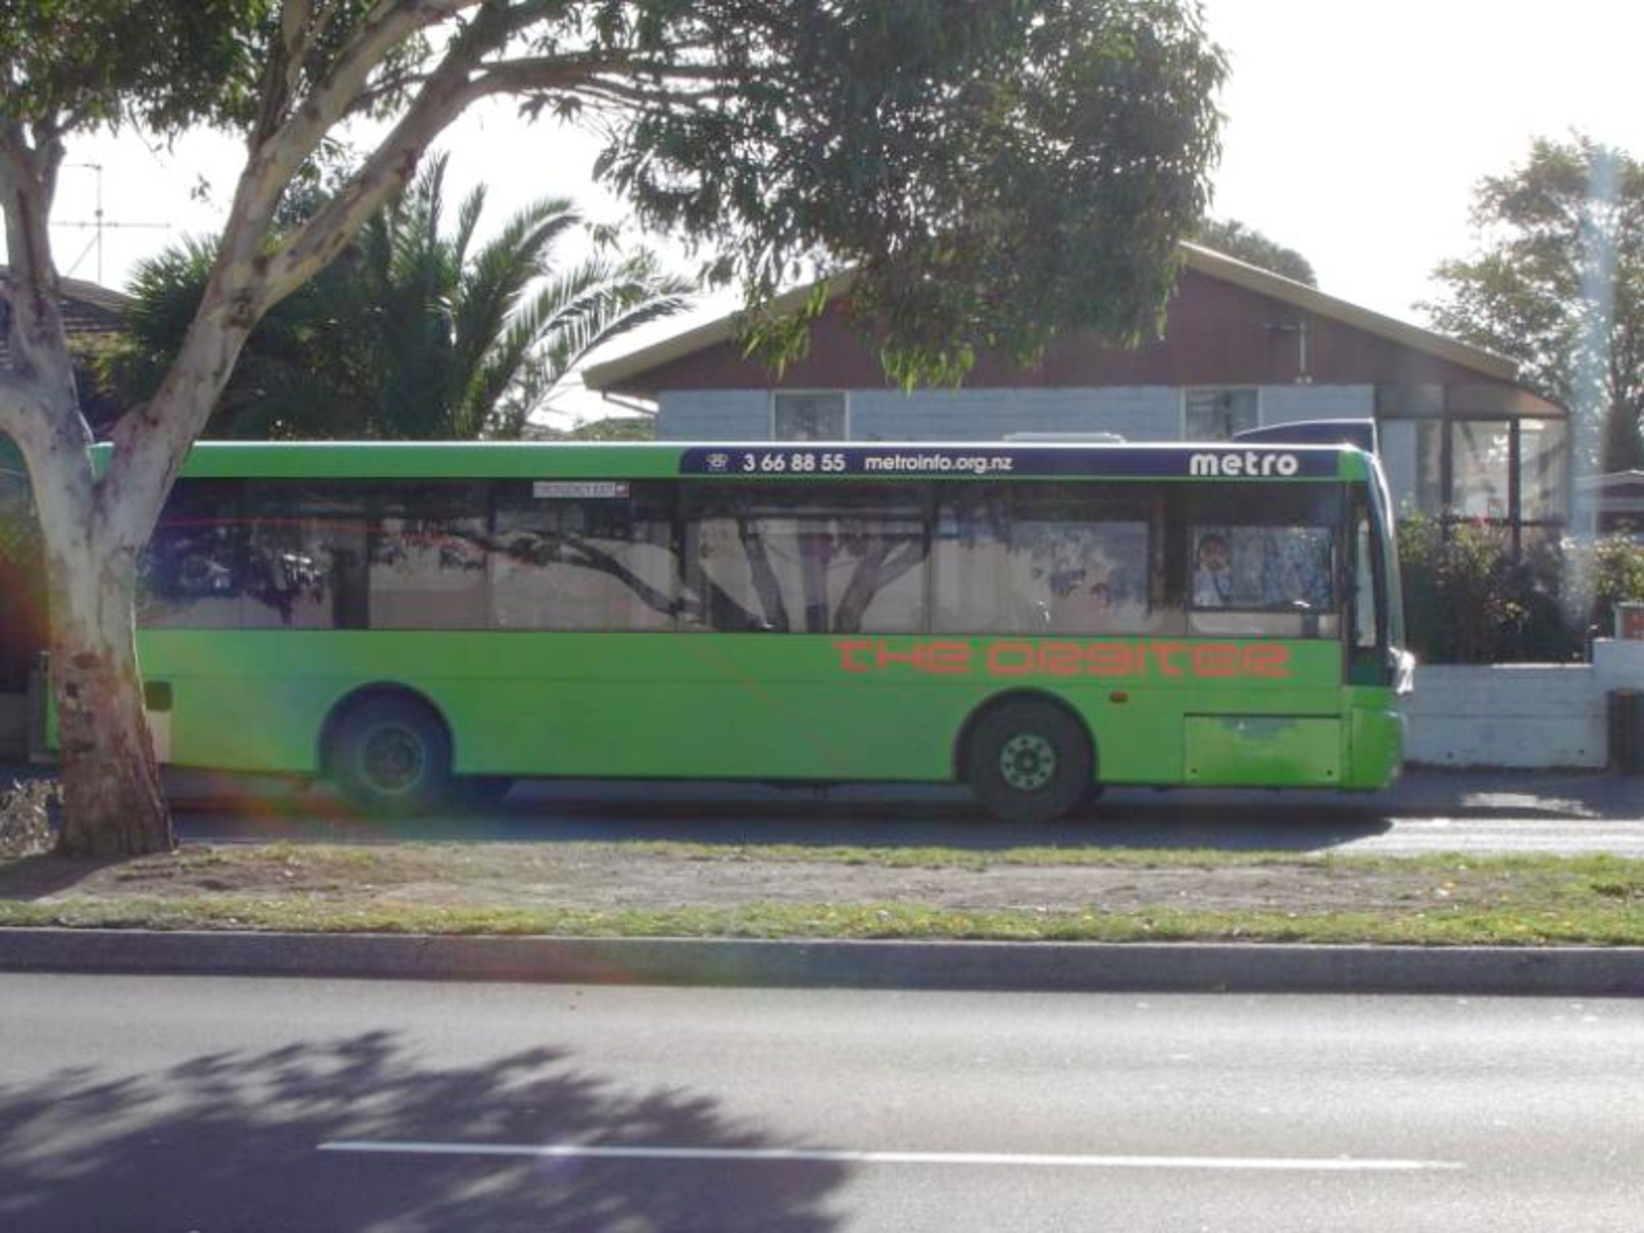
\includegraphics[width=8cm]{figures/OrbiterBus.pdf}
\end{center}

\subsection{Motivation}
The Orbiter is a highly used bus service and I myself often use this service. Many times while waiting for the service, I have noticed that more often than not, two Orbiter buses arrive at the stop at the same time or within a very short time of each other. Because of logistical reasons, I believe the Metro bus company would not run more buses than needed, meaning that if two buses arrived \textquoteleft back to back' then there would be a twenty minute wait for the next bus (as the waiting time should be only ten minutes, so for two buses, the time is doubled.) This type of scenario significantly affects the times specified by Metro. For this reason, I believe that in reality, the average waiting time/arrival time is not ten minutes. It is important to note that the timetables distributed by Metro give specific times when buses arrive. These times are all ten minutes apart, which I feel can only be interpreted as meaning that a bus will arrive at a stop every ten minutes and the maximum waiting time for a passenger is also ten minutes. So for the two buses arriving in the \textquoteleft back to back' situation, while the average time of arrival is presented as every ten minutes on paper, in reality, the buses do not arrive specifically ten minutes apart as claimed. This circumstance also gives a variation of ten minutes and decreases the probability of actually waiting only ten minutes. I wish to address this issue of the average waiting times of the buses in relation to the timetables provided and the variation in actual arrivals. Therefore, by examining the arrival times of the buses and recording waiting times, it can be examined just how accurate the timetables given are and whether they are based on average times or specific times. These issues affect Metro's reliability and credibility.

\subsection{Method}
The experiment we carried out is relatively simple. We sat at the bus stop outside the UCSA building on Ilam road and recorded the arrival times of each Orbiter bus and then calculated the waiting times between each bus. This was done for both clockwise and anticlockwise directions. The waiting time for the first bus in both directions was taken from the time of our arrival to the stop. After that, the waiting time was calculated as the times between bus arrivals.

A range of times were recorded, which covered an entire working day - 8 a.m. to 5 p.m.. These times were recorded on different days to asses not only the time of day but also different days, so we could see how these differeces affect the times. The different times give a fairer assessment of the waiting times. It was assumed that for each day of the week, the waiting times for specific times of the day are relatively the same. A sample taken any day at a specific time would represent all days in the week at that time. The experiment was conducted in this manner because of availability and time restrictions.

While we realise that taking more samples would increase accuracy and reliability while also giving a better description of actual events, we felt it impractical to sit at the stop and record times for an entire day for each day of the week.



\subsubsection*{Statistical Methodology}
For the experiment, we modelled the distribution of the inter-arrival times or waiting times of the Orbiter bus service using the exponential distribution. The probability distribution function is as shown below. The distribution is continuous. $$f(x;\lambda)=\lambda*exp(-\lambda*x)$$
Where: $x$ is the waiting time, and $\lambda$ is the rate parameter or $1/mean(x)$.

The mean of this distribution is $1/\lambda$ and has variance $1/\lambda^2$.

The exponential distribution was chosen because of its important memory-less property. Each new waiting time for the next bus is completely independent of the past waiting times. Each bus's arrival is assumed to be independent of the last.

For this experiment, I will be testing whether the average waiting time is ten minutes. More formally:

\noindent
$\mathbf H_0$(null hypothesis):$\mu=10$ minutes

\noindent
$\mathbf H_A$(Alternative hypothesis):$\mu\neq 10$ minutes


To test this hypothesis, we used non-parametric bootstrap methods to estimate $\lambda$ and obtain a 95\% confidence interval for this value. These values will be formed by sampling the data observed with replacement, at equal probabilities, 132 times, of which an average will be taken. The whole process was then repeated 1000 times. An overall average calculated $\lambda$ will be then transformed into an average waiting time using the formula:$$\mu=1/\lambda$$ where $\mu$ is the average.

This will then be compared and contrasted against the average waiting time found by generating 132 realisations of waiting times then calculating the average of these, then repeating this process 1000 times. This is a parametric bootstrap based technique. For this, $\lambda=1/10$ (where $\mu=10$ minutes and using the formula above.) An overall average will be found along with a 95\% confidence interval for this value. By comparing these intervals and mean values, an accurate decision will be made as to whether buses do arrive on average every ten minutes or not.

Probabilities of certain arrival times around ten minutes will be evaluated to show the accuracy of the service. 

The {\tt Matlab} code for this process is given in Appendix III.

%\newpage
\subsection{Results}
The raw data is given in Appendix IV.
%\newpage

The average waiting time for the anticlockwise direction = 9.19 mins.

The average waiting time for the clockwise direction = 8.95 mins.

The total average = 9.07 mins.

The minimum waiting time = 0 mins.

The maximum waiting time =28 mins.

There are 66 waiting time samples for each direction.

\noindent
{\it Notes for the data:}
\begin{itemize}
    \item Some buses waited at the stop for random amounts of time in order to space the buses apart (this was never for long: 1 or 2 minutes). This was not taken into account when recording arrival times.
\item School rush traffic (heavier volumes) was present from 3 p.m. to 3.30 p.m. approx.
\item Evening commuter rush was present from approx 4.30 p.m. onwards.
\item Morning commuter rush was from 8 a.m. to 9.30 p.m. approx.
\end{itemize}

{\it Observations on the data:}
The anticlockwise direction tends to be much more consistent, having a closer average to ten minutes and more observed times close to ten minutes.
\begin{figure}
\begin{center}
%\includegraphics[width=15cm]{figures/anticlockwise_time.jpg}
%\includegraphics[width=15cm]{figures/clockwise_time.jpg}
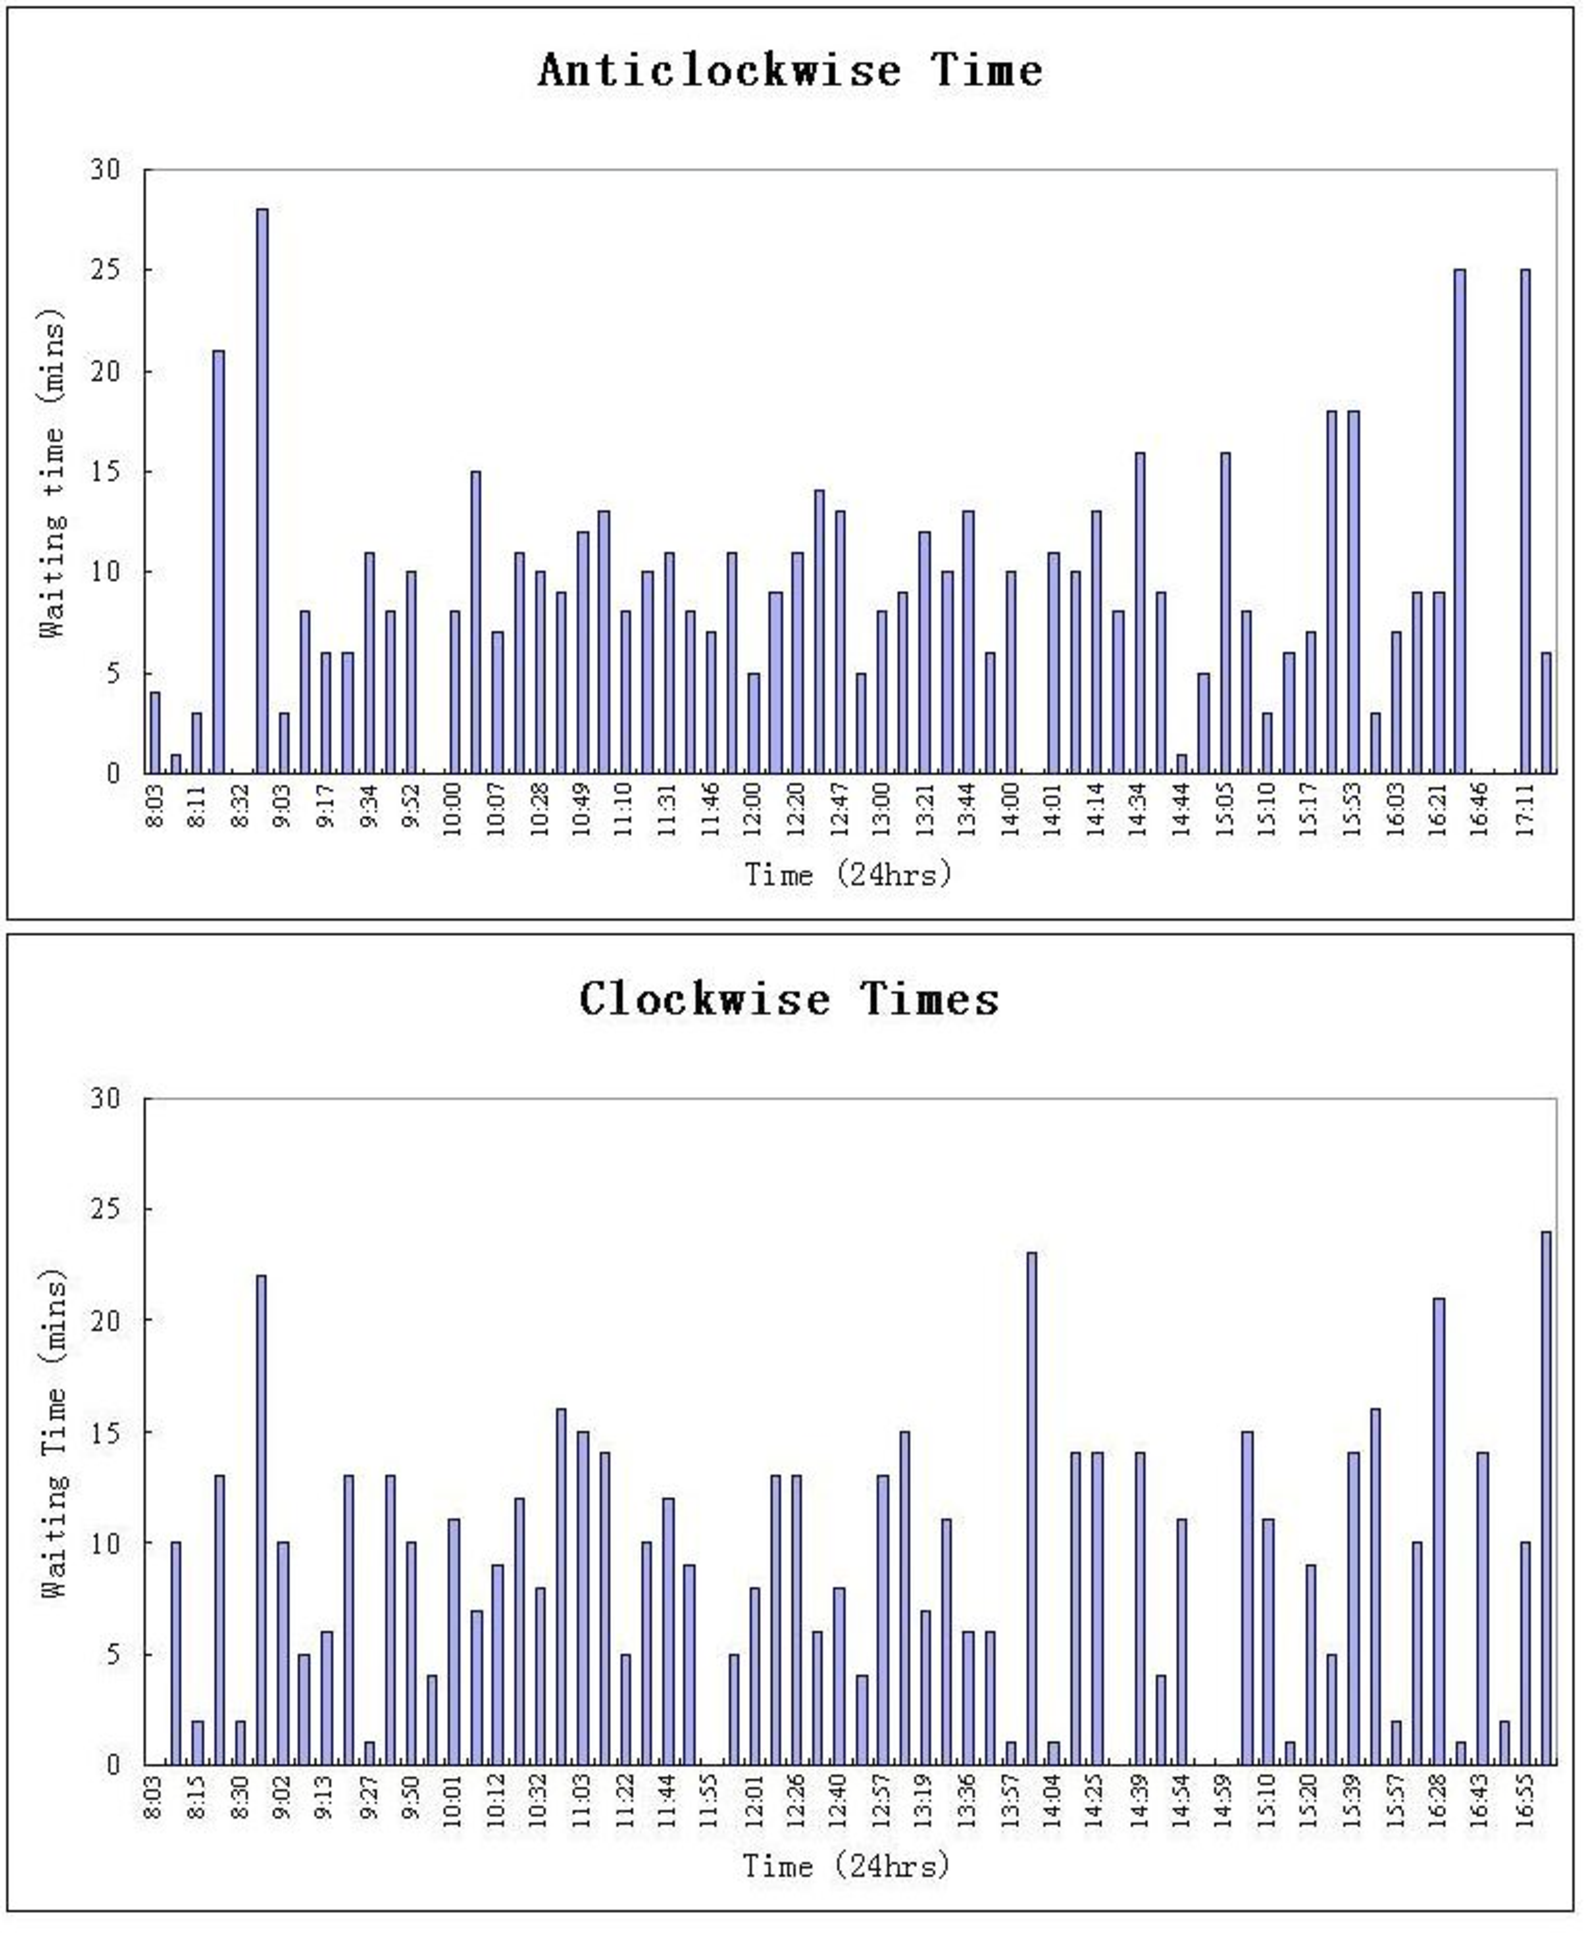
\includegraphics[width=12cm,height=17cm]{figures/OrbiterBusWaitingTimes.pdf}
\caption{From the graphs above, we can see that often, a short wait is followed by a long wait, in both directions. Also, the anticlockwise times are generally much closer to 10 minutes waiting time. It is also seen that around rush hour times (8:30, 15:00, 16:45), a pattern emerged where several buses in quick succession were followed by a long wait for the next bus to arrive. This could be because of the time taken for more passengers than usual to aboard and depart, and areas where traffic volume is greater at these times.}
\end{center}
\end{figure}

\subsection{Discussion}

During less busy hours, buses arrive much more regularly.

The results of the code in (Appendix III) are as follows:

Calculated sample $\lambda=0.1105$. The calculated 95\% confidence interval for this value is [0.1078,0.1129]. The claimed lambda is $\lambda=0.1$. As the calculated sample is within this interval and the claimed $\lambda$ is below, we can see that the bus arrival is slightly less than claimed (using $\mu=1/\lambda$). 

Using the claimed $\lambda$, the randomly obtained mean value for waiting time is $\mu=9.9842$. The calculated 95\% confidence interval for the mean waiting time is [9.2882,10.6237].

I found from the samples that the anticlockwise, clockwise and total mean waiting times are $\mu=$9.19, 8.95 and 9.07, respectively. None of these values is within the interval previously stated.

When the calculated sample $\lambda$ of 0.1105 was used to produce the mean waiting time and its 95\% confidence interval, the following was produced: $\mu$=9.0350 and [8.4957, 9.6137].
\begin{figure}
 \begin{center}
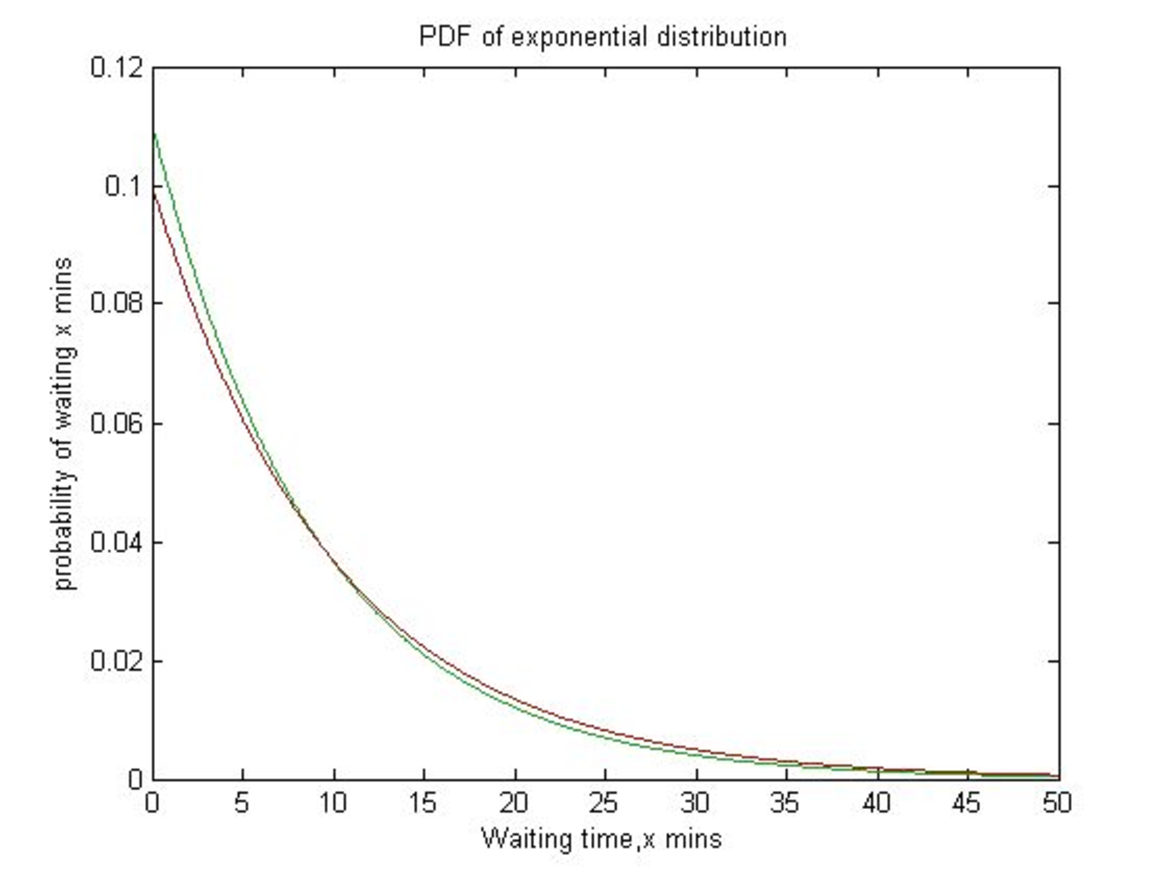
\includegraphics[width=12cm]{figures/OrbiterBus_Pdf_Exp.pdf}
\caption{This graph shows the probability distribution function for the exponential function with the green line indicating a $\lambda$ value of 0.1, the claimed $\lambda$. The red line indicates the value of $\lambda$ estimated, 0.1105. From this graph, you can see the probability of getting a short waiting time is high - approximately 0.06, while the probability of a long waiting time is much much lower - approx imately 0.01. The {\tt Matlab} code for this graph is shown in Appendix I.}
\end{center}
\end{figure}

\begin{figure}
 \begin{center}
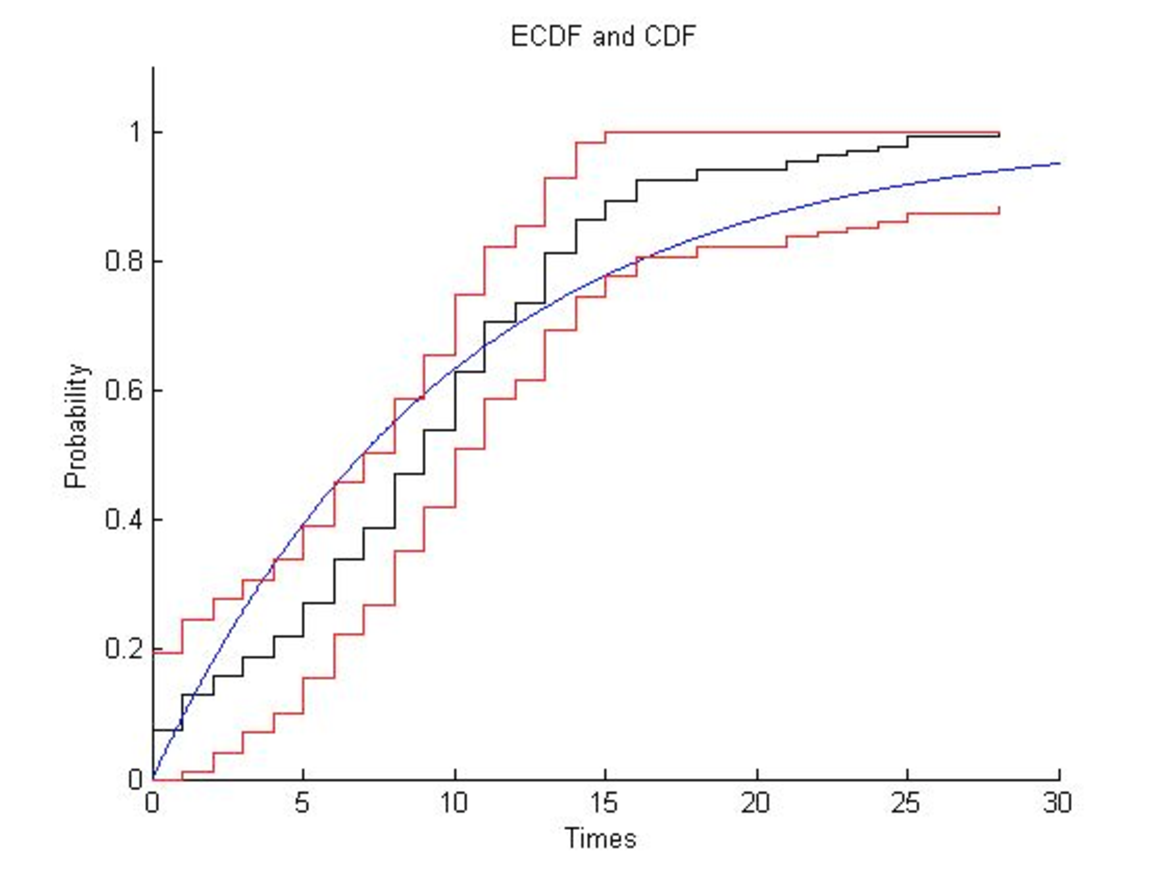
\includegraphics[width=10cm]{figures/OrbiterBus_Ecdf_Cdf.pdf}
\caption{This plot is the Empirical CDF plot(black), with a 95\% confidence interval (red) and the actual CDF based on claimed $\lambda=0.1$ (blue). The {\tt Matlab} code for this graph is given in Appendix II. This graph shows the accuracy of the empirical distribution and hence the accuracy of the data we collected. There are some inconsistencies caused by the randomness of inter-arrival times but our empirical CDF is generally good as the actual CDF lies mostly within the interval lines. With more data points, our accuracy would greatly improve.}
\end{center}
\end{figure}

It is important to note that it is seen in the graph, from the empirical CDF, that the probability of having short waiting times is high - the probability of waiting 10 minutes or less according to our observed data is 6288. This value is quite high but the probability of waiting 15 minutes or more is 0.1288 which, in reality, is relatively high also. Practically, this means 1 in every 10 times you wait for an Orbiter to arrive, it will take 15 minutes or more to come. This value may be acceptable by Metro and indeed is good, considering so many unknown factors in traffic, but it would surely frustrate passengers being 5 minutes behind time. 

\subsection{Conclusion}
The calculated value of $\lambda$ is 0.1105. When this value is used to estimate the mean waiting time, and including the observed waiting times, we can conclude that Metro delivers a service better than claimed. From this $\lambda$, we see a mean waiting time of 9.04 minutes - 58 seconds less than the 10 minutes wait claimed.

Furthermore, the mean waiting time estimate calculated and its 95\% confidence interval (not including the average waiting times observed) cause us to not accept the null hypothesis, $\mathbf H_0$ of $\mu=10$ minutes at the 95\% confidence level.

From all of this, we can confirm that Metro is quite right in claiming an arrival of an Orbiter bus every ten minutes at any stop. In fact, it appears that they do better than this by a whole minute. However, it is all very well to claim this on paper but it is crucial to note that waiting times of 28 minutes do happen, rarely. This illustrates a very important difference between practical and statistical significance. In this case, it has no major effects, as the observed waiting time is less than claimed. 

\subsection*{Author Contributions
%\footnote{Please be aware there is email evidence to prove a lack of comprehension in taks requested of some parties.}%%raaz removed this snide remark however true this may be...June 28 2008
}
{\it Josh's Contributions:} The original concept; data recordings for Wednesday, Thursday and Friday (5hrs); data organisation; analysis; methodology and implementation and the preliminary report, final report and presentation notes.
{\it Yirang's Contributions:} Monday's and Tuesday's data recordings (4hrs).

%\newpage
\subsection*{Appendices}

\subsubsection*{I}
\begin{VrbM}
x=linspace(0,50,1000);%Array of x points to evaluate

lambda1=0.1105%Estimated lambda

f1=lambda1*exp(-lambda1.*x);%Calculated probabilities

plot(x,f1,'color',[0 0.6 0])%Plot coloured red
hold

lambda2=0.1%Claimed lambda

f2=lambda2*exp(-lambda2.*x);%Calculated probabilites

plot(x,f2,'color',[0.6 0 0])%Plot coloured green
xlabel('Waiting time,x mins')%Graph titles
ylabel('probability of waiting x mins')
title('PDF of exponential distribution')
\end{VrbM}
\subsubsection*{II}

\begin{VrbM}
antiTimes=[8 3 7 18 18 3 7 9 9 25 0 0 25 6 ...
  10 0 10 8 16 9 1 5 16 6 4 1 3 21 0 28 3 8 ...
  6 6 11 8 10 15 0 8 7 11 10 9 12 13 8 10 11 8 ...
    7 11 5 9 11 14 13 5 8 9 12 10 13 6 11 13];
clockTimes=[0 0 11 1 9 5 14 16 2 10 21 1 14 2 10 ...
    24 6 1 14 14 0 14 4 11 15 0 10 2 13 2 22 ...
    10 5 6 13 1 13 10 11 4 7 9 12 8 16 15 14 5 ...
    10 12 9 8 0 5 13 13 6 8 4 13 15 7 11 6 23 1];
%The raw data-the waiting times for each direction


sampleTimes=[antiTimes clockTimes];%dd all times into 1 array

x=linspace(0,30,1000);%Create array
lambda1=0.1;%Set claimed lambda
f=1-exp(-lambda1*x);%Create cdf realisations based on claimed lambda

[x1 y1]=ECDF2(sampleTimes,7,0,0);
%Call to class distributed ECDF fuction, save output values in arrays x1
%and y1
hold on%Hold plots for superimposition
plot(x,f)

Alpha=0.05;%set alpha to 5%
SampleSize=132;

Epsn=sqrt((1/(2*SampleSize))*log(2/Alpha));%epsilon_n for the confidence band

stairs(x1,max(y1-Epsn,zeros(1,length(y1))),'r');%lower band plot
stairs(x1,min(y1+Epsn,ones(1,length(y1))),'r');%upper band plot
hold off
axis([0,30,0,1])
title('ECDF and CDF')
xlabel('Times')
ylabel('Probability')
\end{VrbM}
\subsubsection*{III}
\begin{VrbM}
clear
antiTimes=[8 3 7 18 18 3 7 9 9 25 0 0 25 6 ...
  10 0 10 8 16 9 1 5 16 6 4 1 3 21 0 28 3 8 ...
  6 6 11 8 10 15 0 8 7 11 10 9 12 13 8 10 11 8 ...
    7 11 5 9 11 14 13 5 8 9 12 10 13 6 11 13];
clockTimes=[0 0 11 1 9 5 14 16 2 10 21 1 14 2 10 ...
    24 6 1 14 14 0 14 4 11 15 0 10 2 13 2 22 ...
    10 5 6 13 1 13 10 11 4 7 9 12 8 16 15 14 5 ...
    10 12 9 8 0 5 13 13 6 8 4 13 15 7 11 6 23 1];
%The raw data - the waiting times for each direction

rand('twister',489110);%set the seed for rand so results can be reproduced
sampleTimes=[antiTimes clockTimes];%All the sample times collected
lambdaTotal=zeros(1000,1);%An empty array

lambdaObs=1/mean(sampleTimes)%The lambda value for observed samples
lambdaClaimed=1/10 %The lambda claimed by Metro

%This is a non-parametric bootstrap
for j=1:1000%Loop to create 1000 lambdas
    for i=1:132 %A loop to sample with replacement 132 times at equal 
        %probability
        u1=rand;%Generate a random number
        x1=deMoivreEqui(u1,132);%Select a random number between 1 and 132
        b(i)=sampleTimes(x1);%Array of random sample times, taken from 
        %all samples, using random number generated
    end
    lambdaTotal(j)=1/mean(b);%lambda value for each array of random samples
end

sampleLambda=mean(lambdaTotal)
%The mean lambda for all the lambdas calculted
sortedLambdaTotal=sort(lambdaTotal);%Sort lambdas generated
lowerBound=lambdaTotal(25)%Calculate a 95% confidence interval for lambda
upperBound=lambdaTotal(975)

realisationsClaimed=zeros(1000,1);%An empty array
meanClaimed=zeros(1000,1);%An empty array
%This is parametric bootstrap
for x=1:1000%Loop to create 1000 mean waiting times based on claimed lambda
    for z=1:132 %Loop to generate 1000 waiting times based on claimed lambda
        u2=rand;%Generate a random number
        realisationsClaimed(z)=-(1/lambdaClaimed)*log(u2);
        %Create realisation of x, random number u and lambda claimed
    end
    meanClaimed(x)=mean(realisationsClaimed);
    %Find mean of each array of realisations
end
meanOfClaim=mean(meanClaimed)%Overall mean of realisations created
meanClaimed=sort(meanClaimed);%Sort array
lowerBound=meanClaimed(25)
%Create a 95% confidence interval for the mean found
upperBound=meanClaimed(975)
\end{VrbM}

The above code was wtitten 15/10/07 by J Fenemore and makes use of the follwing function:
\begin{VrbM}
function x = deMoivreEqui(u,k);
%
% return samples from deMoivre(1/k,1/k,...,1/k) RV X
%
% File Dates : Created  08/06/07  Modified  08/06/07
% Author(s)  : Raaz 
%
% Call Syntax:  x = deMoivreEqui(u,k);
%               deMoivreEqui(u,k);
%
% Input      : u = array of uniform random numbers e.g. rand 
%              k = number of equi-probabble outcomes of X
% Output     : x = samples from X
%
x = ceil(k * u) ; % ceil(y) is the smallest integer larger than y
% floor is useful when the outcomes are {0,1,...,k-1}
%x = floor(k * u);
%%%%%%%%%%%%%%%%%%%%%%%%%%%%%%%%%%%%%%%%%%%%%%%%%%%%%%
\end{VrbM}
\subsubsection*{IV. Raw data}
{\scriptsize
\begin{table}[tph]
\centering
%\begin{small}
\begin{tabular}{|cc|cc|}\hline
\bf{Anti-clockwise Route}		&		&\bf{Clockwise Route}			&		\\	\hline
Bus Arrival Times:			&	Mins waiting:	&	Bus Arrival Times:			&	Mins waiting:	\\	\hline
15	:	07	&	8	&	14	:	59	&	0	\\	
15	:	10	&	3	&	14	:	59	&	0	\\	
15	:	17	&	7	&	15	:	10	&	11	\\	
15	:	35	&	18	&	15	:	11	&	1	\\	
15	:	53	&	18	&	15	:	20	&	9	\\	
15	:	56	&	3	&	15	:	25	&	5	\\	
16	:	03	&	7	&	15	:	39	&	14	\\	
16	:	12	&	9	&	15	:	55	&	16	\\	
16	:	21	&	9	&	15	:	57	&	2	\\	
16	:	46	&	25	&	16	:	07	&	10	\\	
16	:	46	&	0	&	16	:	28	&	21	\\	
16	:	46	&	0	&	16	:	29	&	1	\\	
17	:	11	&	25	&	16	:	43	&	14	\\	
17	:	17	&	6	&	16	:	45	&	2	\\	
			&		&	16	:	55	&	10	\\	
			&		&	17	:	19	&	24	\\	\hline
14	:	00	&	10	&	13	:	56	&	6	\\	
14	:	00	&	0	&	13	:	57	&	1	\\	
14	:	10	&	10	&	14	:	11	&	14	\\	
14	:	18	&	8	&	14	:	25	&	14	\\	
14	:	34	&	16	&	14	:	25	&	0	\\	
14	:	43	&	9	&	14	:	39	&	14	\\	
14	:	44	&	1	&	14	:	43	&	4	\\	
14	:	49	&	5	&	14	:	54	&	11	\\	
15	:	05	&	16	&	15	:	09	&	15	\\	
15	:	11	&	6	&				&		\\	\hline
8	:	03	&	4	&	8	:	03	&	0	\\	
8	:	08	&	1	&	8	:	13	&	10	\\	
8	:	11	&	3	&	8	:	15	&	2	\\	
8	:	32	&	21	&	8	:	28	&	13	\\	
8	:	32	&	0	&	8	:	30	&	2	\\	
9	:	00	&	28	&	8	:	52	&	22	\\	
9	:	03	&	3	&	9	:	02	&	10	\\	
9	:	11	&	8	&	9	:	07	&	5	\\	
	\hline
\end{tabular}

%\caption{}
%\label{tab:}
\end{table}
\begin{table}[tph]
\centering

\begin{tabular}{|cc|cc|}\hline
\bf{Anti-clockwise Route}		&		&\bf{Clockwise Route}			&		\\	\hline
Bus Arrival Times:			&	Mins waiting:	&	Bus Arrival Times:			&	Mins waiting:	\\	\hline
9	:	17	&	6	&	9	:	13	&	6	\\	
9	:	23	&	6	&	9	:	26	&	13	\\	
9	:	34	&	11	&	9	:	27	&	1	\\	
9	:	42	&	8	&	9	:	40	&	13	\\	
9	:	52	&	10	&	9	:	50	&	10	\\	
10	:	07	&	15	&	10	:	01	&	11	\\\hline
9	:	52	&	0	&	9	:	56	&	4	\\	
10	:	00	&	8	&	10	:	03	&	7	\\	
10	:	07	&	7	&	10	:	12	&	9	\\	
10	:	18	&	11	&	10	:	24	&	12	\\	
10	:	28	&	10	&	10	:	32	&	8	\\	
10	:	37	&	9	&	10	:	48	&	16	\\	
10	:	49	&	12	&	11	:	03	&	15	\\	
11	:	02	&	13	&	11	:	17	&	14	\\	
11	:	10	&	8	&	11	:	22	&	5	\\	
11	:	20	&	10	&	11	:	32	&	10	\\	
11	:	31	&	11	&	11	:	44	&	12	\\	
11	:	39	&	8	&	11	:	53	&	9	\\	
11	:	46	&	7	&	12	:	01	&	8	\\	
11	:	57	&	11	&				&		\\	\hline
12	:	00	&	5	&	11	:	55	&	0	\\	
12	:	09	&	9	&	12	:	00	&	5	\\	
12	:	20	&	11	&	12	:	13	&	13	\\	
12	:	34	&	14	&	12	:	26	&	13	\\	
12	:	47	&	13	&	12	:	32	&	6	\\	
12	:	52	&	5	&	12	:	40	&	8	\\	
13	:	00	&	8	&	12	:	44	&	4	\\	
13	:	09	&	9	&	12	:	57	&	13	\\	
13	:	21	&	12	&	13	:	12	&	15	\\	
13	:	31	&	10	&	13	:	19	&	7	\\	
13	:	44	&	13	&	13	:	30	&	11	\\	
13	:	50	&	6	&	13	:	36	&	6	\\	
14	:	01	&	11	&	13	:	59	&	23	\\	
14	:	14	&	13	&	14	:	04	&	1	\\	\hline
\end{tabular}
%\end{small}
%\caption{}
%\label{tab:}
\end{table}
}
%%%%%%%%%%%%%%%%%%%%%%%%%%%%%%%
\newpage
\section{Diameter of \textit{Dosinia} Shells}
\begin{center}
Guo Yaozong and Shen Chun
\end{center}

\subsection{Introduction and Objective}

We collected some shells from New Brighton Pier that are commonly called \textit{Dosinia anus} (Coarse Venus Shell). This species is a member of the class Bivalivia. Bivalivia lack a radula, and feed by filtering out fine particles of organic matter either from seawater (suspension feeders) or from surface mud (deposit feeders). In each case, food enters the mantle cavity in a current of water produced by cilia on the gills. Gills have a large surface area in relation to the size of the animal, and secrete copious amounts of slime-like mucus that not only traps the food particles but also acts as a lubricant for the passage of food to the mouth. In addition to having this feeding role, gills are the respiratory structures and are richly supplied with blood dorsally. Sexes are separate, although there is no external dimorphism. Gametes are shed into the seawater, where fertilisation occurs.

\begin{figure}[ht]
\begin{center}
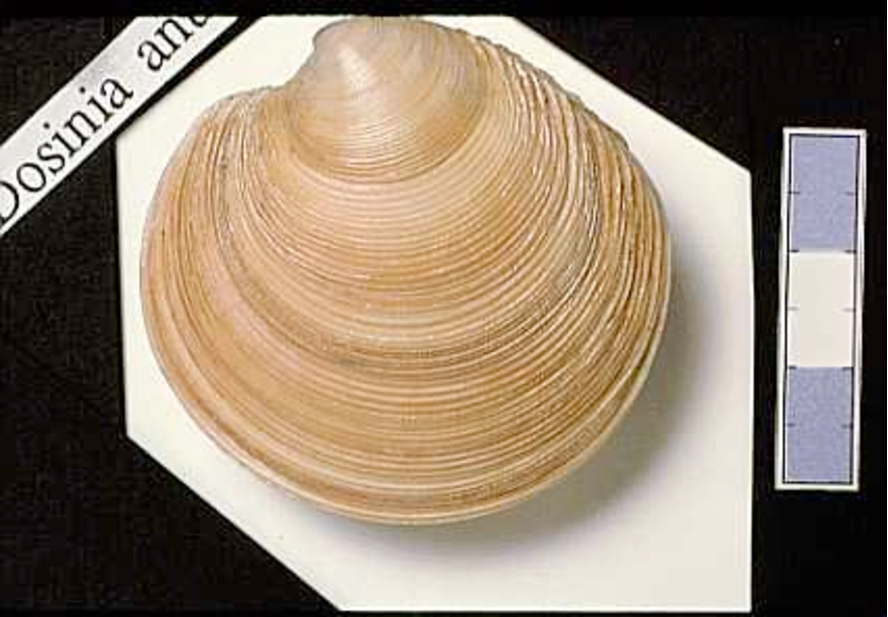
\includegraphics[width=5cm]{figures/DosiniaShellPhoto.pdf}
\end{center}
\end{figure}

Unlike Venus shells from other parts of the world, this species has a flat disc-like shell. Found just below the low-tide mark along Brighton beach, it burrows just below the sand surface and feeds using two short, separate siphons. ({\it Life in The Estuary}, Malcolm B. Jones\& Islay D. Marsden, Canterbury University Press, 2005).

%\section*{Aim}

Our objective was to test whether the diameters of \textit{Dosinia anus} shells on the north side of New Brighton Pier are identically distributed to those found on the south side of the pier.

\subsection{Materials and Methods}

We collected shells along the New Brighton beach to the left (north) and right (south) of the pier. We walked and picked up all the shells we could see, except broken ones. In about two and a half hours, we collected about two buckets of shells from each side of the pier (i.e. two from the left and two from the right). 

After washing, drying and classifying the shells, we found that 254 of them were \textit{Dosinia anus}, 115 collected from north of the pier and 139 from the southern. Then we used mechanical pencils to sketch the outline of each shell onto graph paper and measured the diameter of each in units of millimetres. The way we measured them was from top to bottom (as shown below). After that, we entered the data into a computer, and estimated the empirical CDF as well as confidence bands. 


\subsubsection*{Statistical Methodology }

In order to test the null hypothesis that the shell diameters of our species are identically distributed on both sides of the pier, we applied the non-parametric permutation test. 

By using the permutation test, we tested whether the absolute difference between the two sample means were significantly different from each other.


Step 1: Observe value: T = X(left) - X(right)
                                
Step 2: Combine [ L1 L2 \ldots \ldots \ldots L115 R1\ldots \ldots \ldots R139] '254 Data'

Step 3: Rearrange ({\tt MATLAB} function: 'randperm'):
\begin{displaymath}
\begin{array}{cccc}
           \textrm{ [R110, L45, L78, R2\ldots}& |&\textrm{ \ldots \ldots \ldots L20] } & \textrm{'254 Data'}\\
									\downarrow &&\downarrow\\
                      |\textrm{Mean(1-115)}& --& \textrm{Mean(116-254)}| &= D_i \textrm{(recorded)}\\
		(i = 1, 2, 3 \ldots 10000) &&&
\end{array}
\end{displaymath}


Step 4: Repeat Step 3 10000 times

Step 5: Find out how often 'Di' is greater than 'T', then divided this value by \textbf{10,000}. 
            This is our \textbf{P-value}.

\subsection{Results}

\begin{figure}[ht]
\begin{center}
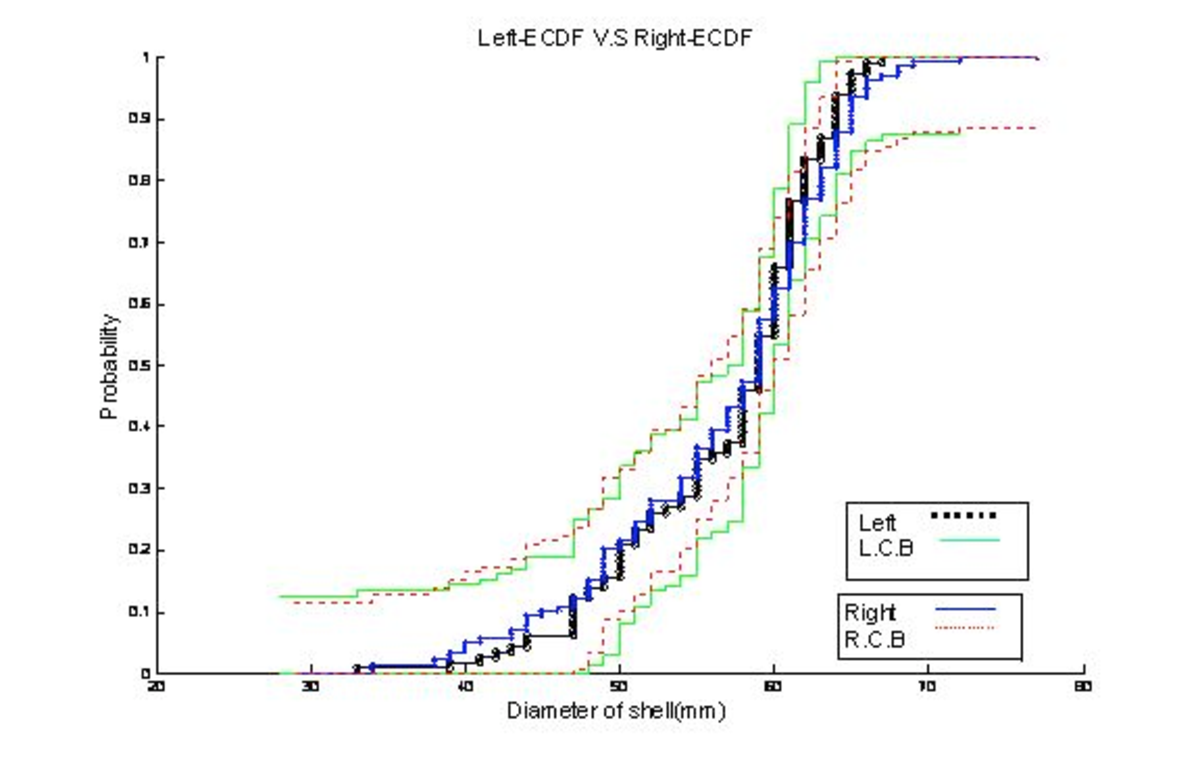
\includegraphics[width=13cm,height=7cm]{figures/DosiniaShell_Left_ECDF_against_Right_ECDF.pdf}
%\includegraphics[width=13cm,height=7cm]{figures/Length_of_shell_against_probability.jpg}
%\caption{A Matlab plot showing the midpoints mapping back to specific values on the x axis}
\end{center}
\end{figure}

\subsubsection*{Hypothesis testing}
abs('mean for north'-'mean for south'): $|56.8173-56.6462|=0.1711 $(observed value)
\textbf{$H_o$}: No difference can be observed between north and south 
\textbf{$H_a$}: A difference can be observed 
Alpha = 0.05

In the test, we found 8470 numbers were greater than 0.1711, so
 P-valve = 8470 / 10000 = 0.847

\subsubsection{Conclusion}
Since p-value is large, we do not reject the null hypothesis, as we do not have enough evidence to say that there is a difference in the distribution of \textit{Dosinia anus} diameters between the north and south sides of the pier in New Brighton Pier.  

\subsection*{Author contributions}

Shen Chun and Yaozong Guo did all the work together.
%%%%%%%%%%%%%%%%%%%%%%%%%%%%%%%
